%%%%%%%%%%%%%%%%%%%%%%%%%%%%%%%%%%%%%%%%%%%%%%%%%%%%%%%%%%%%%%%%%%%%%%%%%%%%%%%%
%
% Template license:
% CC BY-NC-SA 3.0 (http://creativecommons.org/licenses/by-nc-sa/3.0/)
%
%%%%%%%%%%%%%%%%%%%%%%%%%%%%%%%%%%%%%%%%%%%%%%%%%%%%%%%%%%%%%%%%%%%%%%%%%%%%%%%%

%----------------------------------------------------------------------------------------
%	PACKAGES AND OTHER DOCUMENT CONFIGURATIONS
%----------------------------------------------------------------------------------------

\documentclass[
11pt, % The default document font size, options: 10pt, 11pt, 12pt
%oneside, % Two side (alternating margins) for binding by default, uncomment to switch to one side
%chapterinoneline,% Have the chapter title next to the number in one single line
spanish,
singlespacing, % Single line spacing, alternatives: onehalfspacing or doublespacing
%draft, % Uncomment to enable draft mode (no pictures, no links, overfull hboxes indicated)
%nolistspacing, % If the document is onehalfspacing or doublespacing, uncomment this to set spacing in lists to single
%liststotoc, % Uncomment to add the list of figures/tables/etc to the table of contents
%toctotoc, % Uncomment to add the main table of contents to the table of contents
parskip, % Uncomment to add space between paragraphs
%codirector, % Uncomment to add a codirector to the title page
headsepline, % Uncomment to get a line under the header
]{MastersDoctoralThesis} % The class file specifying the document structure



%----------------------------------------------------------------------------------------
%	INFORMACIÓN DE LA MEMORIA
%----------------------------------------------------------------------------------------

\thesistitle{Sistema de monitoreo de servicios de planta} % El títulos de la memoria, se usa en la carátula y se puede usar el cualquier lugar del documento con el comando \ttitle

% Nombre del posgrado, se usa en la carátula y se puede usar el cualquier lugar del documento con el comando \degreename
%\posgrado{Carrera de Especialización en Sistemas Embebidos} 
\posgrado{Carrera de Especialización en Internet de las Cosas} 
%\posgrado{Carrera de Especialización en Intelegencia Artificial}
%\posgrado{Maestría en Sistemas Embebidos} 
%\posgrado{Maestría en Internet de las cosas}

\author{Ing. Marcelo Roberto García} % Tu nombre, se usa en la carátula y se puede usar el cualquier lugar del documento con el comando \authorname

\director{Mg. Ing. Gonzalo Nahuel Vaca (INVAP)} % El nombre del director, se usa en la carátula y se puede usar el cualquier lugar del documento con el comando \dirname
%\codirector{Nombre del codirector (pertenencia)} % El nombre del codirector si lo hubiera, se usa en la carátula y se puede usar el cualquier lugar del documento con el comando \codirname.  Para activar este campo se debe descomentar la opción "codirector" en el comando \documentclass, línea 23.

\juradoUNO{Nombre del jurado 1 (pertenencia)} % Nombre y pertenencia del un jurado se usa en la carátula y se puede usar el cualquier lugar del documento con el comando \jur1name
\juradoDOS{Nombre del jurado 2 (pertenencia)} % Nombre y pertenencia del un jurado se usa en la carátula y se puede usar el cualquier lugar del documento con el comando \jur2name
\juradoTRES{Nombre del jurado 3 (pertenencia)} % Nombre y pertenencia del un jurado se usa en la carátula y se puede usar el cualquier lugar del documento con el comando \jur3name

%\ciudad{Ciudad Autónoma de Buenos Aires}
\ciudad{ciudad de Buenos Aires}

\fechaINICIO{marzo de 2022}
\fechaFINAL{julio de 2023}


\keywords{Sistemas embebidos, FIUBA} % Keywords for your thesis, print it elsewhere with \keywordnames

\usepackage{comment} 
\begin{document}


\frontmatter % Use roman page numbering style (i, ii, iii, iv...) for the pre-content pages

\pagestyle{plain} % Default to the plain heading style until the thesis style is called for the body content


%----------------------------------------------------------------------------------------
%	RESUMEN - ABSTRACT 
%----------------------------------------------------------------------------------------

\begin{abstract}
\addchaptertocentry{\abstractname} % Add the abstract to the table of contents
%
%The Thesis Abstract is written here (and usually kept to just this page). The page is kept centered vertically so can expand into the blank space above the title too\ldots
\centering

  	
La presente memoria describe el desarrollo e implementación de un sistema de recolección de datos de bajo costo enfocado en la optimización del mantenimiento de servicios de planta. El trabajo se realizó para la empresa ROEMMERS S.A.I.C.F en el marco de una propuesta de mejora  por parte del departamento de electrónica con la colaboración del departamento de servicios.

En este trabajo se utilizaron los conocimientos obtenidos de la carrera de especialización en IoT referidos a protocolos de comunicación, tecnologías de backend, frontend, bases de datos, sistemas operativos y redes.


\end{abstract}

%----------------------------------------------------------------------------------------
%	CONTENIDO DE LA MEMORIA  - AGRADECIMIENTOS
%----------------------------------------------------------------------------------------

\begin{acknowledgements}
%\addchaptertocentry{\acknowledgementname} % Descomentando esta línea se puede agregar los agradecimientos al índice
\vspace{1.5cm}

A mi pareja, por su apoyo incondicional.

A mis padres y hermano.

A los profesores, profesoras, compañeros y compañeras por compartir sus conocimientos y experiencias. 

Al Ing. Guillermo Horacio Vidal, Jefe de servicios de laboratorios ROEMMERS, por su confianza.

A Gabriel Méndez, Jefe de mantenimiento electrónico de laboratorios ROEMMERS, por su apoyo.

A todos los que participaron de forma directa e indirecta de este proyecto. 



%\textbf{OPCIONAL}.  

\end{acknowledgements}

%----------------------------------------------------------------------------------------
%	LISTA DE CONTENIDOS/FIGURAS/TABLAS
%----------------------------------------------------------------------------------------

\tableofcontents % Prints the main table of contents

\listoffigures % Prints the list of figures

%\listoftables % Prints the list of tables


%----------------------------------------------------------------------------------------
%	CONTENIDO DE LA MEMORIA  - DEDICATORIA
%----------------------------------------------------------------------------------------

%\dedicatory{\textbf{Dedicado a... Romina Soledad Araujo}}  % escribir acá si se desea una dedicatoria

%----------------------------------------------------------------------------------------
%	CONTENIDO DE LA MEMORIA  - CAPÍTULOS
%----------------------------------------------------------------------------------------

\mainmatter % Begin numeric (1,2,3...) page numbering

\pagestyle{thesis} % Return the page headers back to the "thesis" style

% Incluir los capítulos como archivos separados desde la carpeta Chapters

% Chapter 1

\chapter{Introducción general} % Main chapter title

\label{Chapter1} % For referencing the chapter elsewhere, use \ref{Chapter1} 
\label{IntroGeneral}

%----------------------------------------------------------------------------------------

% Define some commands to keep the formatting separated from the content 
\newcommand{\keyword}[1]{\textbf{#1}}
\newcommand{\tabhead}[1]{\textbf{#1}}
\newcommand{\code}[1]{\texttt{#1}}
\newcommand{\file}[1]{\texttt{\bfseries#1}}
\newcommand{\option}[1]{\texttt{\itshape#1}}
\newcommand{\grados}{$^{\circ}$}

%----------------------------------------------------------------------------------------

%\section{Introducción}

En este capítulo se describen las características del mantenimiento de los servicios de planta, los sistemas de control asociados, su estado del arte, los objetivos y alcances para el desarrollo del siguiente trabajo.

%----------------------------------------------------------------------------------------
\section{Servicios de planta}

Las plantas industriales son las instalaciones por medio del cual es posible la producción de bienes a gran escala, casi la totalidad de los elementos que se consumen, utilizan y desechan a diario provienen o han sido procesados en una planta industrial. 

Este trabajo se encuentra enfocado en una planta farmacéutica donde se producen medicamentos en diversas presentaciones como: sólidos, polvos, efervescentes, líquidos e inyectables.

A continuación se detalla la configuración de una línea de producción de sólidos, esta se encuentra compuesta por una serie de máquinas automáticas donde se recibe el medicamento en polvo para ser comprimido, luego blisteado, estuchado, pesado, etiquetado, apilado y finalmente paletizado.

\begin{figure}[htbp]
	\centering
	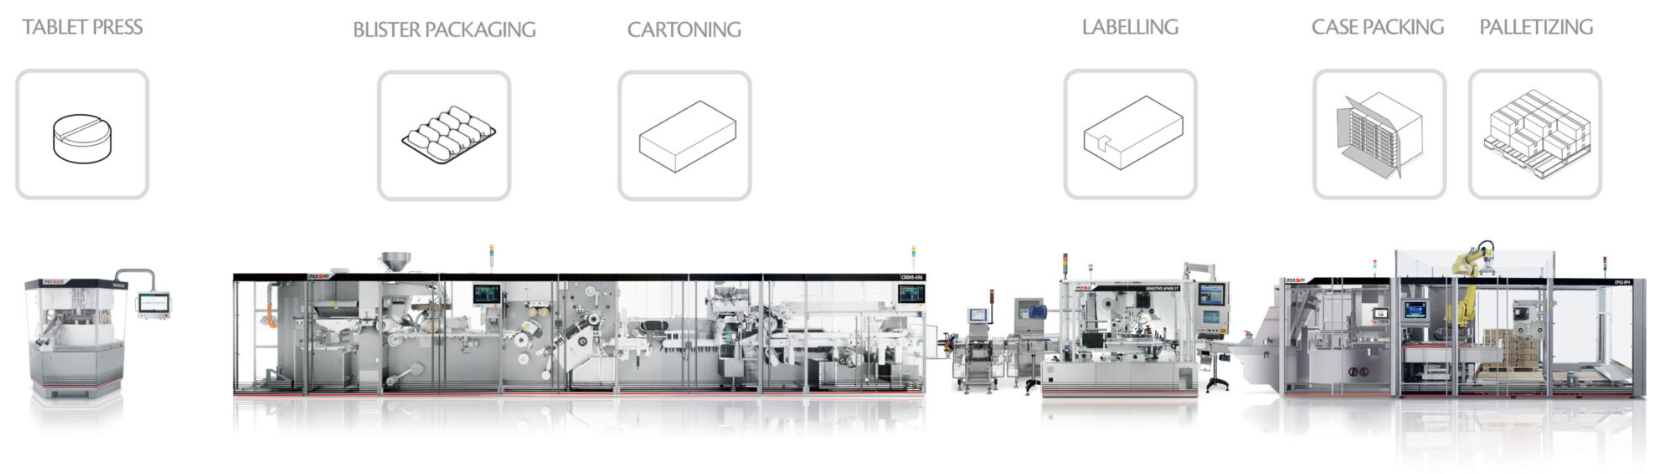
\includegraphics[width=1\textwidth]{./Figures/IMA.png}
	\caption{Linea de blisteado y estuchado.}
	\label{fig:texmaker}
\end{figure}

Las máquinas automáticas cuentan con sistemas de control neumáticos, hidráulicos, térmicos, eléctricos y electrónicos. Estos sistemas requieren servicios esenciales para su funcionamiento como:
 
\begin{itemize}
	\item Electricidad.
	\item Vapor industrial / sanitario
	\item Agua helada / purificada.
	\item Aire comprimido.
\end{itemize}




 

  
%\LaTeX{} no es \textsc{WYSIWYG} (What You See is What You Get), a diferencia de los procesadores de texto como Microsoft Word o Pages de Apple o incluso LibreOffice en el mundo open-source. En lugar de ello, un documento escrito para \LaTeX{} es en realidad un archivo de texto simple o llano que \emph{no contiene formato} . Nosotros le decimos a \LaTeX{} cómo deseamos que se aplique el formato en el documento final escribiendo comandos simples entre el texto, por ejemplo, si quiero usar texto en itálicas para dar énfasis, escribo \verb|\it{texto}| y pongo el texto que quiero en itálicas entre medio de las llaves. Esto significa que \LaTeX{} es un lenguaje del tipo \enquote{mark-up}, muy parecido a HTML.
%\subsection{Una introducción (no tan corta) a \LaTeX{}}

%Si sos nuevo en \LaTeX{}, hay un muy buen libro electrónico - disponible gratuitamente en Internet como un archivo PDF - llamado, \enquote{A (not so short) Introduction to \LaTeX{}}. El título del libro es generalmente acortado a simplemente \emph{lshort}. Puede descargar la versión más reciente en inglés (ya que se actualiza de vez en cuando) desde aquí:
%\url{http://www.ctan.org/tex-archive/info/lshort/english/lshort.pdf}
%
%Se puede encontrar la versión en español en la lista en esta página: \url{http://www.ctan.org/tex-archive/info/lshort/}

%\subsubsection{Una subsubsección}

%Acá tiene un ejemplo de una ``subsubsección'' que es el cuarto nivel de ordenamiento del texto, después de capítulo, sección y subsección.  Como se puede ver, las subsubsecciones no van numeradas en el cuerpo del documento ni en el índice.  El formato está definido por la plantilla y no debe ser modificado.

%\subsection{Guía matemática rápida para \LaTeX{}}

%Si estás escribiendo un documento con mucho contenido matemático, entonces es posible que desees leer el documento de la AMS (American Mathematical Society) llamado, \enquote{A Short Math Guide for \LaTeX{}}. Se puede encontrar en línea en el siguiente link: \url{http://www.ams.org/tex/amslatex.html} en la sección \enquote{Additional Documentation} hacia la parte inferior de la página.


%----------------------------------------------------------------------------------------

\section{Motivación}


Como se ha mencionado anteriormente los servicios de planta deben encontrarse distribuidos por todas las líneas para poder garantizar su funcionamiento.

Considerar HVAC, GMP, CLASIFICACION DE ZONAS para justificar o explicar la motivaciòn.
Autocontrol de la línea operador.


%Si estás familiarizado con \LaTeX{}, entonces podés explorar la estructura de directorios de esta plantilla y proceder a personalizarla agregando tu información en el bloque \emph{INFORMACIÓN DE LA PORTADA} en el archivo \file{memoria.tex}.  
%
%Se puede continuar luego modificando el resto de los archivos siguiendo los lineamientos que se describen en la sección \ref{sec:FillingFile} en la página \pageref{sec:FillingFile}.
%
%Debés asegurarte de leer el capítulo \ref{Chapter2} acerca de las convenciones utilizadas para las Memoria de los Trabajos Finales de la \degreename.
%
%Si sos nuevo en \LaTeX{}, se recomienda que continúes leyendo el documento ya que contiene información básica para aprovechar el potencial de esta herramienta.


%----------------------------------------------------------------------------------------

\section{Estado del arte}

%\subsection{Carpetas}

%Esta plantilla se distribuye como una único archivo .zip que se puede descomprimir en varios archivos y carpetas. Asimismo, se puede consultar el repositorio git para obtener la última versión de los archivos, \url{https://github.com/patriciobos/Plantilla-CESE.git}. Los nombres de las carpetas son, o pretender ser, auto-explicativos.
%
%\keyword{Appendices} -- Esta es la carpeta donde se deben poner los apéndices. Cada apéndice debe ir en su propio archivo \file{.tex}. Se incluye un ejemplo y una plantilla en la carpeta.
%
%\keyword{Chapters} -- Esta es la carpeta donde se deben poner los capítulos de la memoria. Cada capítulo debe ir un su propio archivo \file{.tex} por separado.  Se ofrece por defecto, la siguiente estructura de capítulos y se recomienda su utilización dentro de lo posible:
%
%\begin{itemize}
%\item Capítulo 1: Introducción general	
%\item Capítulo 2: Introducción específica
%\item Capítulo 3: Diseño e implementación
%\item Capítulo 4: Ensayos y resultados
%\item Capítulo 5: Conclusiones
%
%\end{itemize}
%
%Esta estructura de capítulos es la que se recomienda para las memorias de la especialización.
%
%\keyword{Figures} -- Esta carpeta contiene todas las figuras de la memoria.  Estas son las versiones finales de las imágenes que van a ser incluidas en la memoria.  Pueden ser imágenes en formato \textit{raster}\footnote{\url{https://en.wikipedia.org/wiki/Raster_graphics}} como \file{.png}, \file{.jpg} o en formato vectoriales\footnote{\url{https://en.wikipedia.org/wiki/Vector_graphics}} como \file{.pdf}, \file{.ps}.  Se debe notar que utilizar imágenes vectoriales disminuye notablemente el peso del documento final y acelera el tiempo de compilación por lo que es recomendable su utilización siempre que sea posible.

%\subsection{Archivos}

%También están incluidos varios archivos, la mayoría de ellos son de texto plano y se puede ver su contenido en un editor de texto. Después de la compilación inicial, se verá que más archivos auxiliares son creados por \ LaTeX{} o BibTeX, pero son de uso interno y no es necesario hacer nada en particular con ellos.  Toda la información necesaria para compilar el documento se encuentra en los archivos \file{.tex}, \file{.bib}, \file{.cls} y en las imágenes de la carpeta Figures.
%
%\keyword{referencias.bib} - este es un archivo importante que contiene toda la información de referencias bibliográficas que se utilizarán para las citas en la memoria en conjunto con BibTeX. Usted puede escribir las entradas bibliográficas en forma manual, aunque existen también programas de gestión de referencias que facilitan la creación y gestión de las referencias y permiten exportarlas en formato BibTeX.  También hay disponibles sitios web como \url{books.google.com} que permiten obtener toda la información necesaria para una cita en formato BibTeX. Ver sección \ref{sec:biblio}
%
%\keyword{MastersDoctoralThesis.cls} -- este es un archivo importante. Es el archivos con la clase que le informa a \LaTeX{} cómo debe dar formato a la memoria. El usuario de la plantilla no debería necesitar modificar nada de este archivo.
%
%\keyword{memoria.pdf} -- esta es su memoria con una tipografía bellamente compuesta (en formato de archivo PDF) creado por \LaTeX{}. Se distribuye con la plantilla y después de compilar por primera vez sin hacer ningún cambio se debería obtener una versión idéntica a este documento.
%
%\keyword{memoria.tex} -- este es un archivo importante. Este es el archivo que tiene que compilar \LaTeX{} para producir la memoria como un archivo PDF. Contiene un marco de trabajo y estructuras que le indican a \LaTeX{} cómo diagramar la memoria.  Está altamente comentado para que se pueda entender qué es lo que realiza cada línea de código y por qué está incluida en ese lugar.  En este archivo se debe completar la información personalizada de las primeras sección según se indica en la sección \ref{sec:FillingFile}.
%
%Archivos que \emph{no} forman parte de la distribución de la plantilla pero que son generados por \LaTeX{} como archivos auxiliares necesarios para la producción de la memoria.pdf son:
%
%\keyword{memoria.aux} -- este es un archivo auxiliar generado por \LaTeX{}, si se borra \LaTeX{} simplemente lo regenera cuando se compila el archivo principal \file{memoria.tex}.
%
%\keyword{memoria.bbl} -- este es un archivo auxiliar generado por BibTeX, si se borra BibTeX simplemente lo regenera cuando se compila el archivo principal \file{memoria.tex}. Mientras que el archivo \file{.bib} contiene todas las referencias que hay, este archivo \file{.bbl} contine sólo las referencias que han sido citadas y se utiliza para la construcción de la bibiografía.
%
%\keyword{memoria.blg} -- este es un archivo auxiliar generado por BibTeX, si se borra BibTeX simplemente lo regenera cuando se compila el archivo principal \file{memoria.tex}.
%
%\keyword{memoria.lof} -- este es un archivo auxiliar generado por \LaTeX{}, si se borra \LaTeX{} simplemente lo regenera cuando se compila el archivo principal \file{memoria.tex}.  Le indica a \LaTeX{} cómo construir la sección \emph{Lista de Figuras}.
% 
%\keyword{memoria.log} --  este es un archivo auxiliar generado por \LaTeX{}, si se borra \LaTeX{} simplemente lo regenera cuando se compila el archivo principal \file{memoria.tex}. Contiene mensajes de \LaTeX{}. Si se reciben errores o advertencias durante la compilación, se guardan en este archivo \file{.log}.
%
%\keyword{memoria.lot} -- este es un archivo auxiliar generado por \LaTeX{}, si se borra \LaTeX{} simplemente lo regenera cuando se compila el archivo principal \file{memoria.tex}.  Le indica a \LaTeX{} cómo construir la sección \emph{Lista de Tablas}.
%
%\keyword{memoria.out} -- este es un archivo auxiliar generado por \LaTeX{}, si se borra \LaTeX{} simplemente lo regenera cuando se compila el archivo principal \file{memoria.tex}.
%
%De esta larga lista de archivos, sólo aquellos con la extensión \file{.bib}, \file{.cls} y \file{.tex} son importantes.  Los otros archivos auxiliares pueden ser ignorados o borrados ya que \LaTeX{} y BibTeX los regenerarán durante la compilación.

%----------------------------------------------------------------------------------------

\section{Objetivos y alcances}

%Ante de comenzar a editar la plantilla debemos tener un editor \LaTeX{} instalado en nuestra computadora.  En forma análoga a lo que sucede en lenguaje C, que se puede crear y editar código con casi cualquier editor, existen ciertos entornos de trabajo que nos pueden simplificar mucho la tarea.  En este sentido, se recomienda, sobre todo para los principiantes en \LaTeX{} la utilización de TexMaker, un programa gratuito y multi-plantaforma que está disponible tanto para windows como para sistemas GNU/linux.
%
%La versión más reciente de TexMaker es la 4.5 y se puede descargar del siguiente link: \url{http://www.xm1math.net/texmaker/download.html}. Se puede consultar el manual de usuario en el siguiente link: \url{http://www.xm1math.net/texmaker/doc.html}.
 

%\subsection{Paquetes adicionales}

%Si bien durante el proceso de instalación de TexMaker, o cualquier otro editor que se haya elegido, se instalarán en el sistema los paquetes básicos necesarios para trabajar con \LaTeX{}, la plantilla de los trabajos de Especialización y Maestría requieren de paquete adicionales.
%
%Se indican a continuación los comandos que se deben introducir en la consola de Ubuntu (ctrl + alt + t) para instalarlos:
%
%\begin{lstlisting}[language=bash]
%  $ sudo apt install texlive-lang-spanish texlive-science 
%  $ sudo apt install texlive-bibtex-extra biber
%  $ sudo apt install texlive texlive-fonts-recommended
%  $ sudo apt install texlive-latex-extra
%\end{lstlisting}
%

%\subsection{Configurando TexMaker}
\label{subsec:configurando}


%
%Una vez instalado el programa y los paquetes adicionales se debe abrir el archivo memoria.tex con el editor para ver una pantalla similar a la que se puede apreciar en la figura \ref{fig:texmaker}. 
%Una vez instalado el programa y los paquetes adicionales se debe abrir el archivo memoria.tex con el editor para ver una pantalla similar a la que se puede apreciar en la figura \ref{fig:texmaker}. 
%Una vez instalado el programa y los paquetes adicionales se debe abrir el archivo memoria.tex con el editor para ver una pantalla similar a la que se puede apreciar en la figura \ref{fig:texmaker}. 
%Una vez instalado el programa y los paquetes adicionales se debe abrir el archivo memoria.tex con el editor para ver una pantalla similar a la que se puede apreciar en la figura \ref{fig:texmaker}. 
%
%\vspace{1cm}
%
%\begin{figure}[htbp]
%	\centering
%	\includegraphics[width=.5\textwidth]{./Figures/texmaker.png}
%	\caption{Entorno de trabajo de texMaker.}
%	\label{fig:texmaker}
%\end{figure}
%
%\vspace{1cm}
%
%Notar que existe una vista llamada Estructura a la izquierda de la interfaz que nos permite abrir desde dentro del programa los archivos individuales de los capítulos.  A la derecha se encuentra una vista con el archivo propiamente dicho para su edición. Hacia la parte inferior se encuentra una vista del log con información de los resultados de la compilación.  En esta última vista pueden aparecen advertencias o \textit{warning}, que normalmente pueden ser ignorados, y los errores que se indican en color rojo y deben resolverse para que se genere el PDF de salida.
%
%Recordar que el archivo que se debe compilar con PDFLaTeX es \file{memoria.tex}, si se tratara de compilar alguno de los capítulos saldría un error.  Para salvar la molestia de tener que cambiar de archivo para compilar cada vez que se realice una modificación en un capítulo, se puede definir el archivo \file{memoria.tex} como ``documento maestro'' yendo al menú opciones -> ``definir documento actual como documento maestro'', lo que permite compilar con PDFLaTeX memoria.tex directamente desde cualquier archivo que se esté modificando . Se muestra esta opción en la figura \ref{fig:docMaestro}.
%
%\begin{figure}[h]
%	\centering
%	\includegraphics[width=\textwidth]{./Figures/docMaestro.png}
%	\caption{Definir memoria.tex como documento maestro.}
%	\label{fig:docMaestro}
%\end{figure}
%
%En el menú herramientas se encuentran las opciones de compilación.  Para producir un archivo PDF a partir de un archivo .tex se debe ejecutar PDFLaTeX (el shortcut es F6). Para incorporar nueva bibliografía se debe utilizar la opción BibTeX del mismo menú herramientas (el shortcut es F11).
%
%Notar que para actualizar las tablas de contenidos se debe ejecutar PDFLaTeX dos veces.  Esto se debe a que es necesario actualizar algunos archivos auxiliares antes de obtener el resultado final.  En forma similar, para actualizar las referencias bibliográficas se debe ejecutar primero PDFLaTeX, después BibTeX y finalmente PDFLaTeX dos veces por idénticos motivos.

%\section{Personalizando la plantilla, el archivo \file{memoria.tex}}
\label{sec:FillingFile}

%Para personalizar la plantilla se debe incorporar la información propia en los distintos archivos \file{.tex}. 
%
%Primero abrir \file{memoria.tex} con TexMaker (o el editor de su preferencia). Se debe ubicar dentro del archivo el bloque de código titulado \emph{INFORMACIÓN DE LA PORTADA} donde se deben incorporar los primeros datos personales con los que se construirá automáticamente la portada.


%----------------------------------------------------------------------------------------

%\section{El código del archivo \file{memoria.tex} explicado}

%El archivo \file{memoria.tex} contiene la estructura del documento y es el archivo de mayor jerarquía de la memoria.  Podría ser equiparable a la función \emph{main()} de un programa en C, o mejor dicho al archivo fuente .c donde se encuentra definida la función main().
%
%La estructura básica de cualquier documento de \LaTeX{} comienza con la definición de clase del documento, es seguida por un preámbulo donde se pueden agregar funcionalidades con el uso de \texttt{paquetes} (equiparables a bibliotecas de C), y finalmente, termina con el cuerpo del documento, donde irá el contenido de la memoria.
%
%\lstset{%
%  basicstyle=\small\ttfamily,
%  language=[LaTeX]{TeX}
%}
%
%\begin{lstlisting}
%\documentclass{article}  <- Definicion de clase
%\usepackage{listings}	 <- Preambulo
%
%\begin{document}	 <- Comienzo del contenido propio 
%	Hello world!
%\end{document}
%\end{lstlisting}
%
%
%El archivo \file{memoria.tex} se encuentra densamente comentado para explicar qué páginas, secciones y elementos de formato está creando el código \LaTeX{} en cada línea. El código está dividido en bloques con nombres en mayúsculas para que resulte evidente qué es lo que hace esa porción de código en particular. Inicialmente puede parecer que hay mucho código \LaTeX{}, pero es principalmente código para dar formato a la memoria por lo que no requiere intervención del usuario de la plantilla.  Sí se deben personalizar con su información los bloques indicados como:
%
%\begin{itemize}
%	\item Informacion de la memoria
%	\item Resumen
%	\item Agradecimientos
%	\item Dedicatoria
%\end{itemize}
%
%El índice de contenidos, las listas de figura de tablas se generan en forma automática y no requieren intervención ni edición manual por parte del usuario de la plantilla. 
%
%En la parte final del documento se encuentran los capítulos y los apéndices.  Por defecto se incluyen los 5 capítulos propuestos que se encuentran en la carpeta /Chapters. Cada capítulo se debe escribir en un archivo .tex separado y se debe poner en la carpeta \emph{Chapters} con el nombre \file{Chapter1}, \file{Chapter2}, etc\ldots El código para incluir capítulos desde archivos externos se muestra a continuación.
%
%\begin{verbatim}
%	% Chapter 1

\chapter{Introducción general} % Main chapter title

\label{Chapter1} % For referencing the chapter elsewhere, use \ref{Chapter1} 
\label{IntroGeneral}

%----------------------------------------------------------------------------------------

% Define some commands to keep the formatting separated from the content 
\newcommand{\keyword}[1]{\textbf{#1}}
\newcommand{\tabhead}[1]{\textbf{#1}}
\newcommand{\code}[1]{\texttt{#1}}
\newcommand{\file}[1]{\texttt{\bfseries#1}}
\newcommand{\option}[1]{\texttt{\itshape#1}}
\newcommand{\grados}{$^{\circ}$}

%----------------------------------------------------------------------------------------

%\section{Introducción}

En este capítulo se describen las características del mantenimiento de los servicios de planta, los sistemas de control asociados, su estado del arte, los objetivos y alcances para el desarrollo del siguiente trabajo.

%----------------------------------------------------------------------------------------
\section{Servicios de planta}

Las plantas industriales son las instalaciones por medio del cual es posible la producción de bienes a gran escala, casi la totalidad de los elementos que se consumen, utilizan y desechan a diario provienen o han sido procesados en una planta industrial. 

Este trabajo se encuentra enfocado en una planta farmacéutica donde se producen medicamentos en diversas presentaciones como: sólidos, polvos, efervescentes, líquidos e inyectables.

A continuación se detalla la configuración de una línea de producción de sólidos, esta se encuentra compuesta por una serie de máquinas automáticas donde se recibe el medicamento en polvo para ser comprimido, luego blisteado, estuchado, pesado, etiquetado, apilado y finalmente paletizado.

\begin{figure}[htbp]
	\centering
	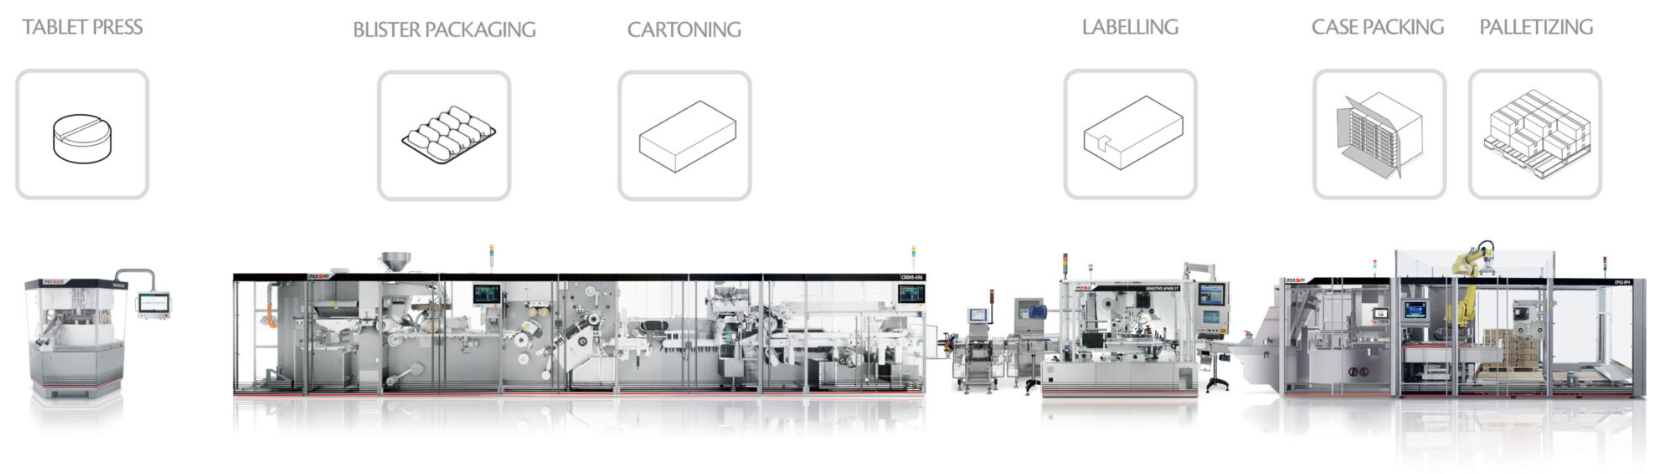
\includegraphics[width=1\textwidth]{./Figures/IMA.png}
	\caption{Linea de blisteado y estuchado.}
	\label{fig:texmaker}
\end{figure}

Las máquinas automáticas cuentan con sistemas de control neumáticos, hidráulicos, térmicos, eléctricos y electrónicos. Estos sistemas requieren servicios esenciales para su funcionamiento como:
 
\begin{itemize}
	\item Electricidad.
	\item Vapor industrial / sanitario
	\item Agua helada / purificada.
	\item Aire comprimido.
\end{itemize}




 

  
%\LaTeX{} no es \textsc{WYSIWYG} (What You See is What You Get), a diferencia de los procesadores de texto como Microsoft Word o Pages de Apple o incluso LibreOffice en el mundo open-source. En lugar de ello, un documento escrito para \LaTeX{} es en realidad un archivo de texto simple o llano que \emph{no contiene formato} . Nosotros le decimos a \LaTeX{} cómo deseamos que se aplique el formato en el documento final escribiendo comandos simples entre el texto, por ejemplo, si quiero usar texto en itálicas para dar énfasis, escribo \verb|\it{texto}| y pongo el texto que quiero en itálicas entre medio de las llaves. Esto significa que \LaTeX{} es un lenguaje del tipo \enquote{mark-up}, muy parecido a HTML.
%\subsection{Una introducción (no tan corta) a \LaTeX{}}

%Si sos nuevo en \LaTeX{}, hay un muy buen libro electrónico - disponible gratuitamente en Internet como un archivo PDF - llamado, \enquote{A (not so short) Introduction to \LaTeX{}}. El título del libro es generalmente acortado a simplemente \emph{lshort}. Puede descargar la versión más reciente en inglés (ya que se actualiza de vez en cuando) desde aquí:
%\url{http://www.ctan.org/tex-archive/info/lshort/english/lshort.pdf}
%
%Se puede encontrar la versión en español en la lista en esta página: \url{http://www.ctan.org/tex-archive/info/lshort/}

%\subsubsection{Una subsubsección}

%Acá tiene un ejemplo de una ``subsubsección'' que es el cuarto nivel de ordenamiento del texto, después de capítulo, sección y subsección.  Como se puede ver, las subsubsecciones no van numeradas en el cuerpo del documento ni en el índice.  El formato está definido por la plantilla y no debe ser modificado.

%\subsection{Guía matemática rápida para \LaTeX{}}

%Si estás escribiendo un documento con mucho contenido matemático, entonces es posible que desees leer el documento de la AMS (American Mathematical Society) llamado, \enquote{A Short Math Guide for \LaTeX{}}. Se puede encontrar en línea en el siguiente link: \url{http://www.ams.org/tex/amslatex.html} en la sección \enquote{Additional Documentation} hacia la parte inferior de la página.


%----------------------------------------------------------------------------------------

\section{Motivación}


Como se ha mencionado anteriormente los servicios de planta deben encontrarse distribuidos por todas las líneas para poder garantizar su funcionamiento.

Considerar HVAC, GMP, CLASIFICACION DE ZONAS para justificar o explicar la motivaciòn.
Autocontrol de la línea operador.


%Si estás familiarizado con \LaTeX{}, entonces podés explorar la estructura de directorios de esta plantilla y proceder a personalizarla agregando tu información en el bloque \emph{INFORMACIÓN DE LA PORTADA} en el archivo \file{memoria.tex}.  
%
%Se puede continuar luego modificando el resto de los archivos siguiendo los lineamientos que se describen en la sección \ref{sec:FillingFile} en la página \pageref{sec:FillingFile}.
%
%Debés asegurarte de leer el capítulo \ref{Chapter2} acerca de las convenciones utilizadas para las Memoria de los Trabajos Finales de la \degreename.
%
%Si sos nuevo en \LaTeX{}, se recomienda que continúes leyendo el documento ya que contiene información básica para aprovechar el potencial de esta herramienta.


%----------------------------------------------------------------------------------------

\section{Estado del arte}

%\subsection{Carpetas}

%Esta plantilla se distribuye como una único archivo .zip que se puede descomprimir en varios archivos y carpetas. Asimismo, se puede consultar el repositorio git para obtener la última versión de los archivos, \url{https://github.com/patriciobos/Plantilla-CESE.git}. Los nombres de las carpetas son, o pretender ser, auto-explicativos.
%
%\keyword{Appendices} -- Esta es la carpeta donde se deben poner los apéndices. Cada apéndice debe ir en su propio archivo \file{.tex}. Se incluye un ejemplo y una plantilla en la carpeta.
%
%\keyword{Chapters} -- Esta es la carpeta donde se deben poner los capítulos de la memoria. Cada capítulo debe ir un su propio archivo \file{.tex} por separado.  Se ofrece por defecto, la siguiente estructura de capítulos y se recomienda su utilización dentro de lo posible:
%
%\begin{itemize}
%\item Capítulo 1: Introducción general	
%\item Capítulo 2: Introducción específica
%\item Capítulo 3: Diseño e implementación
%\item Capítulo 4: Ensayos y resultados
%\item Capítulo 5: Conclusiones
%
%\end{itemize}
%
%Esta estructura de capítulos es la que se recomienda para las memorias de la especialización.
%
%\keyword{Figures} -- Esta carpeta contiene todas las figuras de la memoria.  Estas son las versiones finales de las imágenes que van a ser incluidas en la memoria.  Pueden ser imágenes en formato \textit{raster}\footnote{\url{https://en.wikipedia.org/wiki/Raster_graphics}} como \file{.png}, \file{.jpg} o en formato vectoriales\footnote{\url{https://en.wikipedia.org/wiki/Vector_graphics}} como \file{.pdf}, \file{.ps}.  Se debe notar que utilizar imágenes vectoriales disminuye notablemente el peso del documento final y acelera el tiempo de compilación por lo que es recomendable su utilización siempre que sea posible.

%\subsection{Archivos}

%También están incluidos varios archivos, la mayoría de ellos son de texto plano y se puede ver su contenido en un editor de texto. Después de la compilación inicial, se verá que más archivos auxiliares son creados por \ LaTeX{} o BibTeX, pero son de uso interno y no es necesario hacer nada en particular con ellos.  Toda la información necesaria para compilar el documento se encuentra en los archivos \file{.tex}, \file{.bib}, \file{.cls} y en las imágenes de la carpeta Figures.
%
%\keyword{referencias.bib} - este es un archivo importante que contiene toda la información de referencias bibliográficas que se utilizarán para las citas en la memoria en conjunto con BibTeX. Usted puede escribir las entradas bibliográficas en forma manual, aunque existen también programas de gestión de referencias que facilitan la creación y gestión de las referencias y permiten exportarlas en formato BibTeX.  También hay disponibles sitios web como \url{books.google.com} que permiten obtener toda la información necesaria para una cita en formato BibTeX. Ver sección \ref{sec:biblio}
%
%\keyword{MastersDoctoralThesis.cls} -- este es un archivo importante. Es el archivos con la clase que le informa a \LaTeX{} cómo debe dar formato a la memoria. El usuario de la plantilla no debería necesitar modificar nada de este archivo.
%
%\keyword{memoria.pdf} -- esta es su memoria con una tipografía bellamente compuesta (en formato de archivo PDF) creado por \LaTeX{}. Se distribuye con la plantilla y después de compilar por primera vez sin hacer ningún cambio se debería obtener una versión idéntica a este documento.
%
%\keyword{memoria.tex} -- este es un archivo importante. Este es el archivo que tiene que compilar \LaTeX{} para producir la memoria como un archivo PDF. Contiene un marco de trabajo y estructuras que le indican a \LaTeX{} cómo diagramar la memoria.  Está altamente comentado para que se pueda entender qué es lo que realiza cada línea de código y por qué está incluida en ese lugar.  En este archivo se debe completar la información personalizada de las primeras sección según se indica en la sección \ref{sec:FillingFile}.
%
%Archivos que \emph{no} forman parte de la distribución de la plantilla pero que son generados por \LaTeX{} como archivos auxiliares necesarios para la producción de la memoria.pdf son:
%
%\keyword{memoria.aux} -- este es un archivo auxiliar generado por \LaTeX{}, si se borra \LaTeX{} simplemente lo regenera cuando se compila el archivo principal \file{memoria.tex}.
%
%\keyword{memoria.bbl} -- este es un archivo auxiliar generado por BibTeX, si se borra BibTeX simplemente lo regenera cuando se compila el archivo principal \file{memoria.tex}. Mientras que el archivo \file{.bib} contiene todas las referencias que hay, este archivo \file{.bbl} contine sólo las referencias que han sido citadas y se utiliza para la construcción de la bibiografía.
%
%\keyword{memoria.blg} -- este es un archivo auxiliar generado por BibTeX, si se borra BibTeX simplemente lo regenera cuando se compila el archivo principal \file{memoria.tex}.
%
%\keyword{memoria.lof} -- este es un archivo auxiliar generado por \LaTeX{}, si se borra \LaTeX{} simplemente lo regenera cuando se compila el archivo principal \file{memoria.tex}.  Le indica a \LaTeX{} cómo construir la sección \emph{Lista de Figuras}.
% 
%\keyword{memoria.log} --  este es un archivo auxiliar generado por \LaTeX{}, si se borra \LaTeX{} simplemente lo regenera cuando se compila el archivo principal \file{memoria.tex}. Contiene mensajes de \LaTeX{}. Si se reciben errores o advertencias durante la compilación, se guardan en este archivo \file{.log}.
%
%\keyword{memoria.lot} -- este es un archivo auxiliar generado por \LaTeX{}, si se borra \LaTeX{} simplemente lo regenera cuando se compila el archivo principal \file{memoria.tex}.  Le indica a \LaTeX{} cómo construir la sección \emph{Lista de Tablas}.
%
%\keyword{memoria.out} -- este es un archivo auxiliar generado por \LaTeX{}, si se borra \LaTeX{} simplemente lo regenera cuando se compila el archivo principal \file{memoria.tex}.
%
%De esta larga lista de archivos, sólo aquellos con la extensión \file{.bib}, \file{.cls} y \file{.tex} son importantes.  Los otros archivos auxiliares pueden ser ignorados o borrados ya que \LaTeX{} y BibTeX los regenerarán durante la compilación.

%----------------------------------------------------------------------------------------

\section{Objetivos y alcances}

%Ante de comenzar a editar la plantilla debemos tener un editor \LaTeX{} instalado en nuestra computadora.  En forma análoga a lo que sucede en lenguaje C, que se puede crear y editar código con casi cualquier editor, existen ciertos entornos de trabajo que nos pueden simplificar mucho la tarea.  En este sentido, se recomienda, sobre todo para los principiantes en \LaTeX{} la utilización de TexMaker, un programa gratuito y multi-plantaforma que está disponible tanto para windows como para sistemas GNU/linux.
%
%La versión más reciente de TexMaker es la 4.5 y se puede descargar del siguiente link: \url{http://www.xm1math.net/texmaker/download.html}. Se puede consultar el manual de usuario en el siguiente link: \url{http://www.xm1math.net/texmaker/doc.html}.
 

%\subsection{Paquetes adicionales}

%Si bien durante el proceso de instalación de TexMaker, o cualquier otro editor que se haya elegido, se instalarán en el sistema los paquetes básicos necesarios para trabajar con \LaTeX{}, la plantilla de los trabajos de Especialización y Maestría requieren de paquete adicionales.
%
%Se indican a continuación los comandos que se deben introducir en la consola de Ubuntu (ctrl + alt + t) para instalarlos:
%
%\begin{lstlisting}[language=bash]
%  $ sudo apt install texlive-lang-spanish texlive-science 
%  $ sudo apt install texlive-bibtex-extra biber
%  $ sudo apt install texlive texlive-fonts-recommended
%  $ sudo apt install texlive-latex-extra
%\end{lstlisting}
%

%\subsection{Configurando TexMaker}
\label{subsec:configurando}


%
%Una vez instalado el programa y los paquetes adicionales se debe abrir el archivo memoria.tex con el editor para ver una pantalla similar a la que se puede apreciar en la figura \ref{fig:texmaker}. 
%Una vez instalado el programa y los paquetes adicionales se debe abrir el archivo memoria.tex con el editor para ver una pantalla similar a la que se puede apreciar en la figura \ref{fig:texmaker}. 
%Una vez instalado el programa y los paquetes adicionales se debe abrir el archivo memoria.tex con el editor para ver una pantalla similar a la que se puede apreciar en la figura \ref{fig:texmaker}. 
%Una vez instalado el programa y los paquetes adicionales se debe abrir el archivo memoria.tex con el editor para ver una pantalla similar a la que se puede apreciar en la figura \ref{fig:texmaker}. 
%
%\vspace{1cm}
%
%\begin{figure}[htbp]
%	\centering
%	\includegraphics[width=.5\textwidth]{./Figures/texmaker.png}
%	\caption{Entorno de trabajo de texMaker.}
%	\label{fig:texmaker}
%\end{figure}
%
%\vspace{1cm}
%
%Notar que existe una vista llamada Estructura a la izquierda de la interfaz que nos permite abrir desde dentro del programa los archivos individuales de los capítulos.  A la derecha se encuentra una vista con el archivo propiamente dicho para su edición. Hacia la parte inferior se encuentra una vista del log con información de los resultados de la compilación.  En esta última vista pueden aparecen advertencias o \textit{warning}, que normalmente pueden ser ignorados, y los errores que se indican en color rojo y deben resolverse para que se genere el PDF de salida.
%
%Recordar que el archivo que se debe compilar con PDFLaTeX es \file{memoria.tex}, si se tratara de compilar alguno de los capítulos saldría un error.  Para salvar la molestia de tener que cambiar de archivo para compilar cada vez que se realice una modificación en un capítulo, se puede definir el archivo \file{memoria.tex} como ``documento maestro'' yendo al menú opciones -> ``definir documento actual como documento maestro'', lo que permite compilar con PDFLaTeX memoria.tex directamente desde cualquier archivo que se esté modificando . Se muestra esta opción en la figura \ref{fig:docMaestro}.
%
%\begin{figure}[h]
%	\centering
%	\includegraphics[width=\textwidth]{./Figures/docMaestro.png}
%	\caption{Definir memoria.tex como documento maestro.}
%	\label{fig:docMaestro}
%\end{figure}
%
%En el menú herramientas se encuentran las opciones de compilación.  Para producir un archivo PDF a partir de un archivo .tex se debe ejecutar PDFLaTeX (el shortcut es F6). Para incorporar nueva bibliografía se debe utilizar la opción BibTeX del mismo menú herramientas (el shortcut es F11).
%
%Notar que para actualizar las tablas de contenidos se debe ejecutar PDFLaTeX dos veces.  Esto se debe a que es necesario actualizar algunos archivos auxiliares antes de obtener el resultado final.  En forma similar, para actualizar las referencias bibliográficas se debe ejecutar primero PDFLaTeX, después BibTeX y finalmente PDFLaTeX dos veces por idénticos motivos.

%\section{Personalizando la plantilla, el archivo \file{memoria.tex}}
\label{sec:FillingFile}

%Para personalizar la plantilla se debe incorporar la información propia en los distintos archivos \file{.tex}. 
%
%Primero abrir \file{memoria.tex} con TexMaker (o el editor de su preferencia). Se debe ubicar dentro del archivo el bloque de código titulado \emph{INFORMACIÓN DE LA PORTADA} donde se deben incorporar los primeros datos personales con los que se construirá automáticamente la portada.


%----------------------------------------------------------------------------------------

%\section{El código del archivo \file{memoria.tex} explicado}

%El archivo \file{memoria.tex} contiene la estructura del documento y es el archivo de mayor jerarquía de la memoria.  Podría ser equiparable a la función \emph{main()} de un programa en C, o mejor dicho al archivo fuente .c donde se encuentra definida la función main().
%
%La estructura básica de cualquier documento de \LaTeX{} comienza con la definición de clase del documento, es seguida por un preámbulo donde se pueden agregar funcionalidades con el uso de \texttt{paquetes} (equiparables a bibliotecas de C), y finalmente, termina con el cuerpo del documento, donde irá el contenido de la memoria.
%
%\lstset{%
%  basicstyle=\small\ttfamily,
%  language=[LaTeX]{TeX}
%}
%
%\begin{lstlisting}
%\documentclass{article}  <- Definicion de clase
%\usepackage{listings}	 <- Preambulo
%
%\begin{document}	 <- Comienzo del contenido propio 
%	Hello world!
%\end{document}
%\end{lstlisting}
%
%
%El archivo \file{memoria.tex} se encuentra densamente comentado para explicar qué páginas, secciones y elementos de formato está creando el código \LaTeX{} en cada línea. El código está dividido en bloques con nombres en mayúsculas para que resulte evidente qué es lo que hace esa porción de código en particular. Inicialmente puede parecer que hay mucho código \LaTeX{}, pero es principalmente código para dar formato a la memoria por lo que no requiere intervención del usuario de la plantilla.  Sí se deben personalizar con su información los bloques indicados como:
%
%\begin{itemize}
%	\item Informacion de la memoria
%	\item Resumen
%	\item Agradecimientos
%	\item Dedicatoria
%\end{itemize}
%
%El índice de contenidos, las listas de figura de tablas se generan en forma automática y no requieren intervención ni edición manual por parte del usuario de la plantilla. 
%
%En la parte final del documento se encuentran los capítulos y los apéndices.  Por defecto se incluyen los 5 capítulos propuestos que se encuentran en la carpeta /Chapters. Cada capítulo se debe escribir en un archivo .tex separado y se debe poner en la carpeta \emph{Chapters} con el nombre \file{Chapter1}, \file{Chapter2}, etc\ldots El código para incluir capítulos desde archivos externos se muestra a continuación.
%
%\begin{verbatim}
%	% Chapter 1

\chapter{Introducción general} % Main chapter title

\label{Chapter1} % For referencing the chapter elsewhere, use \ref{Chapter1} 
\label{IntroGeneral}

%----------------------------------------------------------------------------------------

% Define some commands to keep the formatting separated from the content 
\newcommand{\keyword}[1]{\textbf{#1}}
\newcommand{\tabhead}[1]{\textbf{#1}}
\newcommand{\code}[1]{\texttt{#1}}
\newcommand{\file}[1]{\texttt{\bfseries#1}}
\newcommand{\option}[1]{\texttt{\itshape#1}}
\newcommand{\grados}{$^{\circ}$}

%----------------------------------------------------------------------------------------

%\section{Introducción}

En este capítulo se describen las características del mantenimiento de los servicios de planta, los sistemas de control asociados, su estado del arte, los objetivos y alcances para el desarrollo del siguiente trabajo.

%----------------------------------------------------------------------------------------
\section{Servicios de planta}

Las plantas industriales son las instalaciones por medio del cual es posible la producción de bienes a gran escala, casi la totalidad de los elementos que se consumen, utilizan y desechan a diario provienen o han sido procesados en una planta industrial. 

Este trabajo se encuentra enfocado en una planta farmacéutica donde se producen medicamentos en diversas presentaciones como: sólidos, polvos, efervescentes, líquidos e inyectables.

A continuación se detalla la configuración de una línea de producción de sólidos, esta se encuentra compuesta por una serie de máquinas automáticas donde se recibe el medicamento en polvo para ser comprimido, luego blisteado, estuchado, pesado, etiquetado, apilado y finalmente paletizado.

\begin{figure}[htbp]
	\centering
	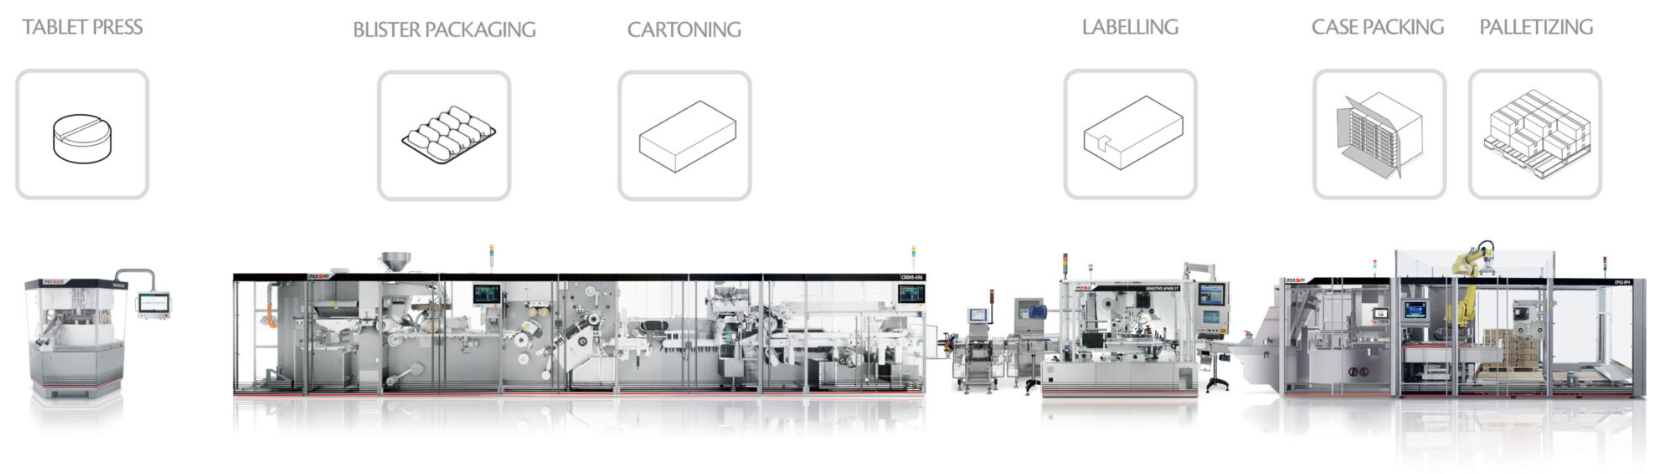
\includegraphics[width=1\textwidth]{./Figures/IMA.png}
	\caption{Linea de blisteado y estuchado.}
	\label{fig:texmaker}
\end{figure}

Las máquinas automáticas cuentan con sistemas de control neumáticos, hidráulicos, térmicos, eléctricos y electrónicos. Estos sistemas requieren servicios esenciales para su funcionamiento como:
 
\begin{itemize}
	\item Electricidad.
	\item Vapor industrial / sanitario
	\item Agua helada / purificada.
	\item Aire comprimido.
\end{itemize}




 

  
%\LaTeX{} no es \textsc{WYSIWYG} (What You See is What You Get), a diferencia de los procesadores de texto como Microsoft Word o Pages de Apple o incluso LibreOffice en el mundo open-source. En lugar de ello, un documento escrito para \LaTeX{} es en realidad un archivo de texto simple o llano que \emph{no contiene formato} . Nosotros le decimos a \LaTeX{} cómo deseamos que se aplique el formato en el documento final escribiendo comandos simples entre el texto, por ejemplo, si quiero usar texto en itálicas para dar énfasis, escribo \verb|\it{texto}| y pongo el texto que quiero en itálicas entre medio de las llaves. Esto significa que \LaTeX{} es un lenguaje del tipo \enquote{mark-up}, muy parecido a HTML.
%\subsection{Una introducción (no tan corta) a \LaTeX{}}

%Si sos nuevo en \LaTeX{}, hay un muy buen libro electrónico - disponible gratuitamente en Internet como un archivo PDF - llamado, \enquote{A (not so short) Introduction to \LaTeX{}}. El título del libro es generalmente acortado a simplemente \emph{lshort}. Puede descargar la versión más reciente en inglés (ya que se actualiza de vez en cuando) desde aquí:
%\url{http://www.ctan.org/tex-archive/info/lshort/english/lshort.pdf}
%
%Se puede encontrar la versión en español en la lista en esta página: \url{http://www.ctan.org/tex-archive/info/lshort/}

%\subsubsection{Una subsubsección}

%Acá tiene un ejemplo de una ``subsubsección'' que es el cuarto nivel de ordenamiento del texto, después de capítulo, sección y subsección.  Como se puede ver, las subsubsecciones no van numeradas en el cuerpo del documento ni en el índice.  El formato está definido por la plantilla y no debe ser modificado.

%\subsection{Guía matemática rápida para \LaTeX{}}

%Si estás escribiendo un documento con mucho contenido matemático, entonces es posible que desees leer el documento de la AMS (American Mathematical Society) llamado, \enquote{A Short Math Guide for \LaTeX{}}. Se puede encontrar en línea en el siguiente link: \url{http://www.ams.org/tex/amslatex.html} en la sección \enquote{Additional Documentation} hacia la parte inferior de la página.


%----------------------------------------------------------------------------------------

\section{Motivación}


Como se ha mencionado anteriormente los servicios de planta deben encontrarse distribuidos por todas las líneas para poder garantizar su funcionamiento.

Considerar HVAC, GMP, CLASIFICACION DE ZONAS para justificar o explicar la motivaciòn.
Autocontrol de la línea operador.


%Si estás familiarizado con \LaTeX{}, entonces podés explorar la estructura de directorios de esta plantilla y proceder a personalizarla agregando tu información en el bloque \emph{INFORMACIÓN DE LA PORTADA} en el archivo \file{memoria.tex}.  
%
%Se puede continuar luego modificando el resto de los archivos siguiendo los lineamientos que se describen en la sección \ref{sec:FillingFile} en la página \pageref{sec:FillingFile}.
%
%Debés asegurarte de leer el capítulo \ref{Chapter2} acerca de las convenciones utilizadas para las Memoria de los Trabajos Finales de la \degreename.
%
%Si sos nuevo en \LaTeX{}, se recomienda que continúes leyendo el documento ya que contiene información básica para aprovechar el potencial de esta herramienta.


%----------------------------------------------------------------------------------------

\section{Estado del arte}

%\subsection{Carpetas}

%Esta plantilla se distribuye como una único archivo .zip que se puede descomprimir en varios archivos y carpetas. Asimismo, se puede consultar el repositorio git para obtener la última versión de los archivos, \url{https://github.com/patriciobos/Plantilla-CESE.git}. Los nombres de las carpetas son, o pretender ser, auto-explicativos.
%
%\keyword{Appendices} -- Esta es la carpeta donde se deben poner los apéndices. Cada apéndice debe ir en su propio archivo \file{.tex}. Se incluye un ejemplo y una plantilla en la carpeta.
%
%\keyword{Chapters} -- Esta es la carpeta donde se deben poner los capítulos de la memoria. Cada capítulo debe ir un su propio archivo \file{.tex} por separado.  Se ofrece por defecto, la siguiente estructura de capítulos y se recomienda su utilización dentro de lo posible:
%
%\begin{itemize}
%\item Capítulo 1: Introducción general	
%\item Capítulo 2: Introducción específica
%\item Capítulo 3: Diseño e implementación
%\item Capítulo 4: Ensayos y resultados
%\item Capítulo 5: Conclusiones
%
%\end{itemize}
%
%Esta estructura de capítulos es la que se recomienda para las memorias de la especialización.
%
%\keyword{Figures} -- Esta carpeta contiene todas las figuras de la memoria.  Estas son las versiones finales de las imágenes que van a ser incluidas en la memoria.  Pueden ser imágenes en formato \textit{raster}\footnote{\url{https://en.wikipedia.org/wiki/Raster_graphics}} como \file{.png}, \file{.jpg} o en formato vectoriales\footnote{\url{https://en.wikipedia.org/wiki/Vector_graphics}} como \file{.pdf}, \file{.ps}.  Se debe notar que utilizar imágenes vectoriales disminuye notablemente el peso del documento final y acelera el tiempo de compilación por lo que es recomendable su utilización siempre que sea posible.

%\subsection{Archivos}

%También están incluidos varios archivos, la mayoría de ellos son de texto plano y se puede ver su contenido en un editor de texto. Después de la compilación inicial, se verá que más archivos auxiliares son creados por \ LaTeX{} o BibTeX, pero son de uso interno y no es necesario hacer nada en particular con ellos.  Toda la información necesaria para compilar el documento se encuentra en los archivos \file{.tex}, \file{.bib}, \file{.cls} y en las imágenes de la carpeta Figures.
%
%\keyword{referencias.bib} - este es un archivo importante que contiene toda la información de referencias bibliográficas que se utilizarán para las citas en la memoria en conjunto con BibTeX. Usted puede escribir las entradas bibliográficas en forma manual, aunque existen también programas de gestión de referencias que facilitan la creación y gestión de las referencias y permiten exportarlas en formato BibTeX.  También hay disponibles sitios web como \url{books.google.com} que permiten obtener toda la información necesaria para una cita en formato BibTeX. Ver sección \ref{sec:biblio}
%
%\keyword{MastersDoctoralThesis.cls} -- este es un archivo importante. Es el archivos con la clase que le informa a \LaTeX{} cómo debe dar formato a la memoria. El usuario de la plantilla no debería necesitar modificar nada de este archivo.
%
%\keyword{memoria.pdf} -- esta es su memoria con una tipografía bellamente compuesta (en formato de archivo PDF) creado por \LaTeX{}. Se distribuye con la plantilla y después de compilar por primera vez sin hacer ningún cambio se debería obtener una versión idéntica a este documento.
%
%\keyword{memoria.tex} -- este es un archivo importante. Este es el archivo que tiene que compilar \LaTeX{} para producir la memoria como un archivo PDF. Contiene un marco de trabajo y estructuras que le indican a \LaTeX{} cómo diagramar la memoria.  Está altamente comentado para que se pueda entender qué es lo que realiza cada línea de código y por qué está incluida en ese lugar.  En este archivo se debe completar la información personalizada de las primeras sección según se indica en la sección \ref{sec:FillingFile}.
%
%Archivos que \emph{no} forman parte de la distribución de la plantilla pero que son generados por \LaTeX{} como archivos auxiliares necesarios para la producción de la memoria.pdf son:
%
%\keyword{memoria.aux} -- este es un archivo auxiliar generado por \LaTeX{}, si se borra \LaTeX{} simplemente lo regenera cuando se compila el archivo principal \file{memoria.tex}.
%
%\keyword{memoria.bbl} -- este es un archivo auxiliar generado por BibTeX, si se borra BibTeX simplemente lo regenera cuando se compila el archivo principal \file{memoria.tex}. Mientras que el archivo \file{.bib} contiene todas las referencias que hay, este archivo \file{.bbl} contine sólo las referencias que han sido citadas y se utiliza para la construcción de la bibiografía.
%
%\keyword{memoria.blg} -- este es un archivo auxiliar generado por BibTeX, si se borra BibTeX simplemente lo regenera cuando se compila el archivo principal \file{memoria.tex}.
%
%\keyword{memoria.lof} -- este es un archivo auxiliar generado por \LaTeX{}, si se borra \LaTeX{} simplemente lo regenera cuando se compila el archivo principal \file{memoria.tex}.  Le indica a \LaTeX{} cómo construir la sección \emph{Lista de Figuras}.
% 
%\keyword{memoria.log} --  este es un archivo auxiliar generado por \LaTeX{}, si se borra \LaTeX{} simplemente lo regenera cuando se compila el archivo principal \file{memoria.tex}. Contiene mensajes de \LaTeX{}. Si se reciben errores o advertencias durante la compilación, se guardan en este archivo \file{.log}.
%
%\keyword{memoria.lot} -- este es un archivo auxiliar generado por \LaTeX{}, si se borra \LaTeX{} simplemente lo regenera cuando se compila el archivo principal \file{memoria.tex}.  Le indica a \LaTeX{} cómo construir la sección \emph{Lista de Tablas}.
%
%\keyword{memoria.out} -- este es un archivo auxiliar generado por \LaTeX{}, si se borra \LaTeX{} simplemente lo regenera cuando se compila el archivo principal \file{memoria.tex}.
%
%De esta larga lista de archivos, sólo aquellos con la extensión \file{.bib}, \file{.cls} y \file{.tex} son importantes.  Los otros archivos auxiliares pueden ser ignorados o borrados ya que \LaTeX{} y BibTeX los regenerarán durante la compilación.

%----------------------------------------------------------------------------------------

\section{Objetivos y alcances}

%Ante de comenzar a editar la plantilla debemos tener un editor \LaTeX{} instalado en nuestra computadora.  En forma análoga a lo que sucede en lenguaje C, que se puede crear y editar código con casi cualquier editor, existen ciertos entornos de trabajo que nos pueden simplificar mucho la tarea.  En este sentido, se recomienda, sobre todo para los principiantes en \LaTeX{} la utilización de TexMaker, un programa gratuito y multi-plantaforma que está disponible tanto para windows como para sistemas GNU/linux.
%
%La versión más reciente de TexMaker es la 4.5 y se puede descargar del siguiente link: \url{http://www.xm1math.net/texmaker/download.html}. Se puede consultar el manual de usuario en el siguiente link: \url{http://www.xm1math.net/texmaker/doc.html}.
 

%\subsection{Paquetes adicionales}

%Si bien durante el proceso de instalación de TexMaker, o cualquier otro editor que se haya elegido, se instalarán en el sistema los paquetes básicos necesarios para trabajar con \LaTeX{}, la plantilla de los trabajos de Especialización y Maestría requieren de paquete adicionales.
%
%Se indican a continuación los comandos que se deben introducir en la consola de Ubuntu (ctrl + alt + t) para instalarlos:
%
%\begin{lstlisting}[language=bash]
%  $ sudo apt install texlive-lang-spanish texlive-science 
%  $ sudo apt install texlive-bibtex-extra biber
%  $ sudo apt install texlive texlive-fonts-recommended
%  $ sudo apt install texlive-latex-extra
%\end{lstlisting}
%

%\subsection{Configurando TexMaker}
\label{subsec:configurando}


%
%Una vez instalado el programa y los paquetes adicionales se debe abrir el archivo memoria.tex con el editor para ver una pantalla similar a la que se puede apreciar en la figura \ref{fig:texmaker}. 
%Una vez instalado el programa y los paquetes adicionales se debe abrir el archivo memoria.tex con el editor para ver una pantalla similar a la que se puede apreciar en la figura \ref{fig:texmaker}. 
%Una vez instalado el programa y los paquetes adicionales se debe abrir el archivo memoria.tex con el editor para ver una pantalla similar a la que se puede apreciar en la figura \ref{fig:texmaker}. 
%Una vez instalado el programa y los paquetes adicionales se debe abrir el archivo memoria.tex con el editor para ver una pantalla similar a la que se puede apreciar en la figura \ref{fig:texmaker}. 
%
%\vspace{1cm}
%
%\begin{figure}[htbp]
%	\centering
%	\includegraphics[width=.5\textwidth]{./Figures/texmaker.png}
%	\caption{Entorno de trabajo de texMaker.}
%	\label{fig:texmaker}
%\end{figure}
%
%\vspace{1cm}
%
%Notar que existe una vista llamada Estructura a la izquierda de la interfaz que nos permite abrir desde dentro del programa los archivos individuales de los capítulos.  A la derecha se encuentra una vista con el archivo propiamente dicho para su edición. Hacia la parte inferior se encuentra una vista del log con información de los resultados de la compilación.  En esta última vista pueden aparecen advertencias o \textit{warning}, que normalmente pueden ser ignorados, y los errores que se indican en color rojo y deben resolverse para que se genere el PDF de salida.
%
%Recordar que el archivo que se debe compilar con PDFLaTeX es \file{memoria.tex}, si se tratara de compilar alguno de los capítulos saldría un error.  Para salvar la molestia de tener que cambiar de archivo para compilar cada vez que se realice una modificación en un capítulo, se puede definir el archivo \file{memoria.tex} como ``documento maestro'' yendo al menú opciones -> ``definir documento actual como documento maestro'', lo que permite compilar con PDFLaTeX memoria.tex directamente desde cualquier archivo que se esté modificando . Se muestra esta opción en la figura \ref{fig:docMaestro}.
%
%\begin{figure}[h]
%	\centering
%	\includegraphics[width=\textwidth]{./Figures/docMaestro.png}
%	\caption{Definir memoria.tex como documento maestro.}
%	\label{fig:docMaestro}
%\end{figure}
%
%En el menú herramientas se encuentran las opciones de compilación.  Para producir un archivo PDF a partir de un archivo .tex se debe ejecutar PDFLaTeX (el shortcut es F6). Para incorporar nueva bibliografía se debe utilizar la opción BibTeX del mismo menú herramientas (el shortcut es F11).
%
%Notar que para actualizar las tablas de contenidos se debe ejecutar PDFLaTeX dos veces.  Esto se debe a que es necesario actualizar algunos archivos auxiliares antes de obtener el resultado final.  En forma similar, para actualizar las referencias bibliográficas se debe ejecutar primero PDFLaTeX, después BibTeX y finalmente PDFLaTeX dos veces por idénticos motivos.

%\section{Personalizando la plantilla, el archivo \file{memoria.tex}}
\label{sec:FillingFile}

%Para personalizar la plantilla se debe incorporar la información propia en los distintos archivos \file{.tex}. 
%
%Primero abrir \file{memoria.tex} con TexMaker (o el editor de su preferencia). Se debe ubicar dentro del archivo el bloque de código titulado \emph{INFORMACIÓN DE LA PORTADA} donde se deben incorporar los primeros datos personales con los que se construirá automáticamente la portada.


%----------------------------------------------------------------------------------------

%\section{El código del archivo \file{memoria.tex} explicado}

%El archivo \file{memoria.tex} contiene la estructura del documento y es el archivo de mayor jerarquía de la memoria.  Podría ser equiparable a la función \emph{main()} de un programa en C, o mejor dicho al archivo fuente .c donde se encuentra definida la función main().
%
%La estructura básica de cualquier documento de \LaTeX{} comienza con la definición de clase del documento, es seguida por un preámbulo donde se pueden agregar funcionalidades con el uso de \texttt{paquetes} (equiparables a bibliotecas de C), y finalmente, termina con el cuerpo del documento, donde irá el contenido de la memoria.
%
%\lstset{%
%  basicstyle=\small\ttfamily,
%  language=[LaTeX]{TeX}
%}
%
%\begin{lstlisting}
%\documentclass{article}  <- Definicion de clase
%\usepackage{listings}	 <- Preambulo
%
%\begin{document}	 <- Comienzo del contenido propio 
%	Hello world!
%\end{document}
%\end{lstlisting}
%
%
%El archivo \file{memoria.tex} se encuentra densamente comentado para explicar qué páginas, secciones y elementos de formato está creando el código \LaTeX{} en cada línea. El código está dividido en bloques con nombres en mayúsculas para que resulte evidente qué es lo que hace esa porción de código en particular. Inicialmente puede parecer que hay mucho código \LaTeX{}, pero es principalmente código para dar formato a la memoria por lo que no requiere intervención del usuario de la plantilla.  Sí se deben personalizar con su información los bloques indicados como:
%
%\begin{itemize}
%	\item Informacion de la memoria
%	\item Resumen
%	\item Agradecimientos
%	\item Dedicatoria
%\end{itemize}
%
%El índice de contenidos, las listas de figura de tablas se generan en forma automática y no requieren intervención ni edición manual por parte del usuario de la plantilla. 
%
%En la parte final del documento se encuentran los capítulos y los apéndices.  Por defecto se incluyen los 5 capítulos propuestos que se encuentran en la carpeta /Chapters. Cada capítulo se debe escribir en un archivo .tex separado y se debe poner en la carpeta \emph{Chapters} con el nombre \file{Chapter1}, \file{Chapter2}, etc\ldots El código para incluir capítulos desde archivos externos se muestra a continuación.
%
%\begin{verbatim}
%	\include{Chapters/Chapter1}
%	\include{Chapters/Chapter2} 
%	\include{Chapters/Chapter3}
%	\include{Chapters/Chapter4} 
%	\include{Chapters/Chapter5} 
%\end{verbatim}
%
%Los apéndices también deben escribirse en archivos .tex separados, que se deben ubicar dentro de la carpeta \emph{Appendices}. Los apéndices vienen comentados por defecto con el caracter \code{\%} y para incluirlos simplemente se debe eliminar dicho caracter.
%
%Finalmente, se encuentra el código para incluir la bibliografía en el documento final.  Este código tampoco debe modificarse. La metodología para trabajar las referencias bibliográficas se desarrolla en la sección \ref{sec:biblio}.
%----------------------------------------------------------------------------------------

%\section{Bibliografía}
%\label{sec:biblio}
%
%Las opciones de formato de la bibliografía se controlan a través del paquete de latex \option{biblatex} que se incluye en la memoria en el archivo memoria.tex.  Estas opciones determinan cómo se generan las citas bibliográficas en el cuerpo del documento y cómo se genera la bibliografía al final de la memoria.
%
%En el preámbulo se puede encontrar el código que incluye el paquete biblatex, que no requiere ninguna modificación del usuario de la plantilla, y que contiene las siguientes opciones:
%
%\begin{lstlisting}
%\usepackage[backend=bibtex,
%	natbib=true, 
%	style=numeric, 
%	sorting=none]
%{biblatex}
%\end{lstlisting}
%
%En el archivo \file{reference.bib} se encuentran las referencias bibliográficas que se pueden citar en el documento.  Para incorporar una nueva cita al documento lo primero es agregarla en este archivo con todos los campos necesario.  Todas las entradas bibliográficas comienzan con $@$ y una palabra que define el formato de la entrada.  Para cada formato existen campos obligatorios que deben completarse. No importa el orden en que las entradas estén definidas en el archivo .bib.  Tampoco es importante el orden en que estén definidos los campos de una entrada bibliográfica. A continuación se muestran algunos ejemplos:
%
%\begin{lstlisting}
%@ARTICLE{ARTICLE:1,
%    AUTHOR="John Doe",
%    TITLE="Title",
%    JOURNAL="Journal",
%    YEAR="2017",
%}
%\end{lstlisting}
%
%
%\begin{lstlisting}
%@BOOK{BOOK:1,
%    AUTHOR="John Doe",
%    TITLE="The Book without Title",
%    PUBLISHER="Dummy Publisher",
%    YEAR="2100",
%}
%\end{lstlisting}
%
%
%\begin{lstlisting}
%@INBOOK{BOOK:2,
%    AUTHOR="John Doe",
%    TITLE="The Book without Title",
%    PUBLISHER="Dummy Publisher",
%    YEAR="2100",
%    PAGES="100-200",
%}
%\end{lstlisting}
%
%
%\begin{lstlisting}
%@MISC{WEBSITE:1,
%    HOWPUBLISHED = "\url{http://example.com}",
%    AUTHOR = "Intel",
%    TITLE = "Example Website",
%    MONTH = "12",
%    YEAR = "1988",
%    URLDATE = {2012-11-26}
%}
%\end{lstlisting}
%
%Se debe notar que los nombres \emph{ARTICLE:1}, \emph{BOOK:1}, \emph{BOOK:2} y \emph{WEBSITE:1} son nombres de fantasía que le sirve al autor del documento para identificar la entrada. En este sentido, se podrían reemplazar por cualquier otro nombre.  Tampoco es necesario poner : seguido de un número, en los ejemplos sólo se incluye como un posible estilo para identificar las entradas.
%
%La entradas se citan en el documento con el comando: 
%
%\begin{verbatim}
%\citep{nombre_de_la_entrada}
%\end{verbatim}
%
%Y cuando se usan, se muestran así: \citep{ARTICLE:1}, \citep{BOOK:1}, \citep{BOOK:2}, \citep{WEBSITE:1}.  Notar cómo se conforma la sección Bibliografía al final del documento.
%
%Finalmente y como se mencionó en la subsección \ref{subsec:configurando}, para actualizar las referencias bibliográficas tanto en la sección bibliografía como las citas en el cuerpo del documento, se deben ejecutar las herramientas de compilación PDFLaTeX, BibTeX, PDFLaTeX, PDFLaTeX, en ese orden.  Este procedimiento debería resolver cualquier mensaje "Citation xxxxx on page x undefined".

%	\chapter{Introducción específica} % Main chapter title

\label{Chapter2}

%----------------------------------------------------------------------------------------
%	SECTION 1
%----------------------------------------------------------------------------------------
En el siguiente capitulo se realiza una introducción a las tecnológicas utilizadas en el desarrollo de este trabajo. Estas tecnologías se aplican a lo largo de las distintas capas del modelo de arquitectura IoT (\textit{Internet of Things})
\section{Protocolos de comunicación}
\label{sec:ejemplo}

Los protocolos de comunicación son estándares que se utilizar para definir de que manera se vinculan uno o mas dispositivos. Existen una gran cantidad de protocolos, estos resuelven distintas problemáticas, a continuación se detallan los utilizados en el desarrollo de este trabajo.

\subsection{SPI \textit{Serial Peripherical Interface}}

EL protocolo de comunicación SPI es un protocolo de comunicación serie que se caracteriza por ser sincrónico y \textit{full duplex}.
Su comunicación se realiza mediante 4 hilos como se observa en la figura \ref{fig:SPI} .

\begin{figure}[htbp]
	\centering
	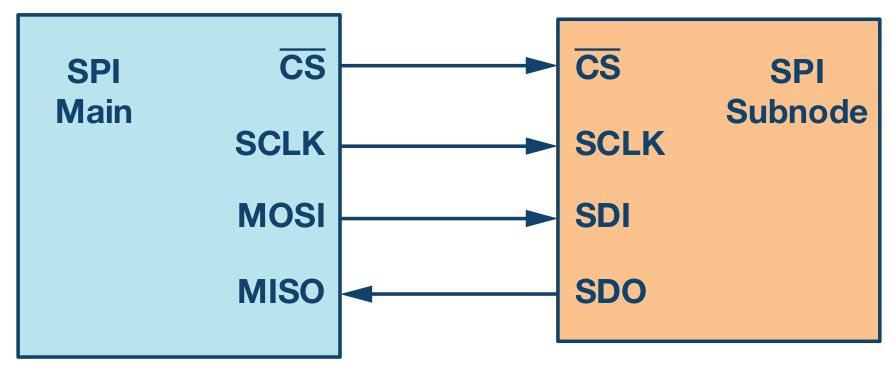
\includegraphics[width=0.6\textwidth]{./Figures/SPI.png}
	\caption{Conexión entre dispositivos SPI.\protect\footnotemark.}
	\label{fig:SPI}
\end{figure} 

Los dispositivos SPI pueden ser direccionables mediante las señales de CS \textit{chip select} y alcanzar velocidades de reloj de hasta 50MHz. 

Esto permite la comunicación entre dispositivos que transfieren un gran cantidad de datos como displays, modulos ethernet y memorias entre otros. 


\subsection{I2C \textit{Inter Integrated Circuit}}

I2C es un protocolo de comunicación serie  bidireccional con un número reducido de hilos para su conexión. Como puede observarse en la figura \ref{fig:I2C}, solo se necesitan dos cables para conectar una serie de dispositivos.

\begin{figure}[htbp]
	\centering
	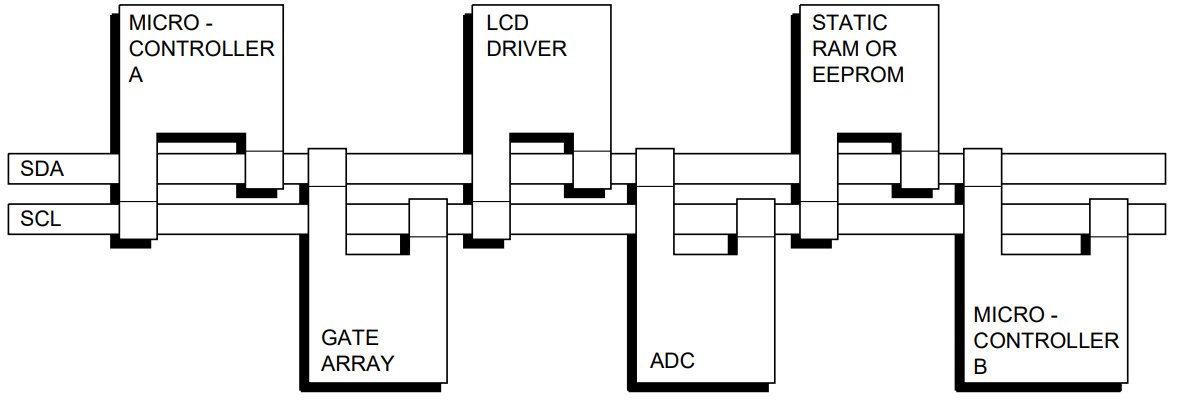
\includegraphics[width=0.8\textwidth]{./Figures/I2C.png}
	\caption{Conexión entre dispositivos I2C.\protect\footnotemark.}
	\label{fig:I2C}
\end{figure} 

Soporta un rango de velocidades desde los 100 kHz a los 5MHz, es direccionable y cuenta con dispositivos para aplicaciones, militares, medicinales e industriales.

Entre los más utilizados se pueden encontrar, memorias, ADC, DAC, sensores de temperatura y humedad, giróscopos electrónicos, etc.

\subsection{UART \textit{Universal Asincronous Receiver Transmitter}}

El protocolo de comunicación serie UART es uno de los más antiguos y utilizados en la comunicación entre dispositivos. Este protocolo es asincrónico, por lo que no cuenta una señal de clock, esta característica reduce la cantidad de hilos de conexión como se detalla en la Figura \ref{fig:UART}


\begin{figure}[htbp]
	\centering
	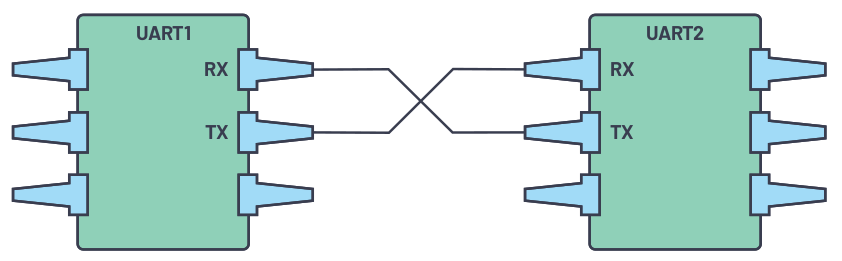
\includegraphics[width=0.6\textwidth]{./Figures/UART.png}
	\caption{Conexión entre dispositivos UART.\protect\footnotemark.}
	\label{fig:UART}
\end{figure} 

A diferencias de los protocolos I2C y  SPI, este no soporta direccionamiento, y su velocidad de comunicación es muy inferior en comparación a los anteriores. Dedido a su sencillez y bajo costo el mismo se continúa utilizando en algunos dispositivos como, módulos WiFi, módulos LoRa, interfaz de comunicación a PC e impresoras.

\subsection{LoRa \textit{Long Range}}

LoRa es una tecnología de comunicación inalámbrica que utiliza la modulación CSS(\textit{Chip Spread Spectrum}) desarrollada por la empresa Semtech. 
La utilización de este tipo de modulación posee grandes ventajas de alcance, inmunidad al ruido y consumo.
En la figura \ref{fig:LoRa} se observa la forma de onda modulada de un dispositivo LoRa. 

\begin{figure}[htbp]
	\centering
	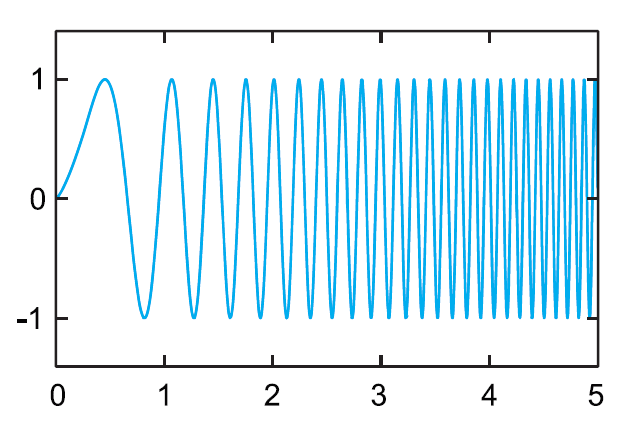
\includegraphics[width=0.3\textwidth]{./Figures/LoRa.png}
	\caption{Modulación CSS.\protect\footnotemark.}
	\label{fig:LoRa}
\end{figure} 

Los dispositivos LoRa utilizan el espectro de frecuencias no licenciado ISM ( \textit{Industrial, Scientific and Medical}) de 915 MHz para el caso de nuestro país, esto reduce el costo operativo de la instalación de dispositivos con esta tecnología.

Con la incorporación del \textit{stack} LoRaWAN, esta tecnología se ha convertido en una de las mas populares en el ecosistema IoT.


\subsection{ModBUS TCP}

Modbus es un protocolo de aplicación abierto Maestro/Esclavo que se puede utilizar en distintas capas físicas. 
Modbus TCP significa que el protocolo Modbus se utiliza en la parte superior de Ethernet TCP/IP, un protocolo orientado a la conexión con el que se busca asegurar la entrega de datos.

\begin{figure}[htbp]
	\centering
	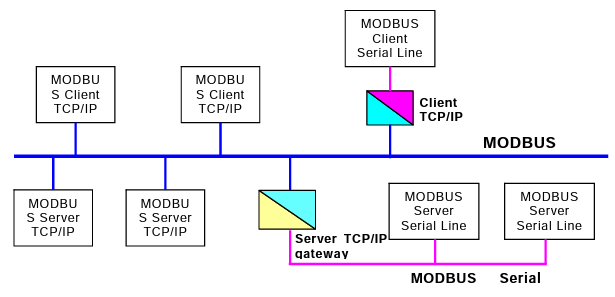
\includegraphics[width=0.7\textwidth]{./Figures/ModBUS.png}
	\caption{Arquitectura de comunicación ModBUS TCP.\protect\footnotemark.}
	\label{fig:ModBUS}
\end{figure} 

Este protocolo ha sido adoptado en la industria por una gran cantidad de fabricantes y en dispositivos controladores lógicos programables, interfase hombre máquina, sensores, actuadores, variadores de velocidad, etc.

ModBUS es un protocolo sencillo, económico y de rápida implementación. Dada su integración existente en los distintos componentes industriales, es muy utilizado cuando se requiere obtener datos de dispositivos industriales. 

\subsection{HTTP \textit{Hypertext Transfer Protocol}}

HTTP es un protocolo de la capa de aplicación para la transmisión de documentos hipermedia, como HTML \textit{HyperText Markup Language} del tipo cliente - servidor. 
Es un protocolo del tipo cliente - servidor, en el que un cliente establece una conexión con el servidor, realiza una petición y espera hasta que recibe una respuesta.

\subsection{Wi-Fi}

\subsection{MQTT}


%\subsection{Uso de mayúscula inicial para los título de secciones}

Si en el texto se hace alusión a diferentes partes del trabajo referirse a ellas como capítulo, sección o subsección según corresponda. Por ejemplo: ``En el capítulo \ref{Chapter1} se explica tal cosa'', o ``En la sección \ref{sec:ejemplo} se presenta lo que sea'', o ``En la subsección \ref{subsec:ejemplo} se discute otra cosa''.

Cuando se quiere poner una lista tabulada, se hace así:

\begin{itemize}
	\item Este es el primer elemento de la lista.
	\item Este es el segundo elemento de la lista.
\end{itemize}

Notar el uso de las mayúsculas y el punto al final de cada elemento.

Si se desea poner una lista numerada el formato es este:

\begin{enumerate}
	\item Este es el primer elemento de la lista.
	\item Este es el segundo elemento de la lista.
\end{enumerate}

Notar el uso de las mayúsculas y el punto al final de cada elemento.

\section{Tecnologías de backend}
\label{subsec:ejemplo}

Se recomienda no utilizar \textbf{texto en negritas} en ningún párrafo, ni tampoco texto \underline{subrayado}. En cambio sí se debe utilizar \textit{texto en itálicas} para palabras en un idioma extranjero, al menos la primera vez que aparecen en el texto. En el caso de palabras que estamos inventando se deben utilizar ``comillas'', así como también para citas textuales. Por ejemplo, un \textit{digital filter} es una especie de ``selector'' que permite separar ciertos componentes armónicos en particular.

La escritura debe ser impersonal. Por ejemplo, no utilizar ``el diseño del firmware lo hice de acuerdo con tal principio'', sino ``el firmware fue diseñado utilizando tal principio''. 

El trabajo es algo que al momento de escribir la memoria se supone que ya está concluido, entonces todo lo que se refiera a hacer el trabajo se narra en tiempo pasado, porque es algo que ya ocurrió. Por ejemplo, "se diseñó el firmware empleando la técnica de test driven development".

En cambio, la memoria es algo que está vivo cada vez que el lector la lee. Por eso transcurre siempre en tiempo presente, como por ejemplo:

``En el presente capítulo se da una visión global sobre las distintas pruebas realizadas y los resultados obtenidos. Se explica el modo en que fueron llevados a cabo los test unitarios y las pruebas del sistema''.

Se recomienda no utilizar una sección de glosario sino colocar la descripción de las abreviaturas como parte del mismo cuerpo del texto. Por ejemplo, RTOS (\textit{Real Time Operating System}, Sistema Operativo de Tiempo Real) o en caso de considerarlo apropiado mediante notas a pie de página.

Si se desea indicar alguna página web utilizar el siguiente formato de referencias bibliográficas, dónde las referencias se detallan en la sección de bibliografía de la memoria, utilizado el formato establecido por IEEE en \citep{IEEE:citation}. Por ejemplo, ``el presente trabajo se basa en la plataforma EDU-CIAA-NXP \citep{CIAA}, la cual...''.

\section{Tecnologías de frontend} 

Al insertar figuras en la memoria se deben considerar determinadas pautas. Para empezar, usar siempre tipografía claramente legible. Luego, tener claro que \textbf{es incorrecto} escribir por ejemplo esto: ``El diseño elegido es un cuadrado, como se ve en la siguiente figura:''

\begin{figure}[h]
\centering
\includegraphics[scale=.45]{./Figures/cuadradoAzul.png}
\end{figure}

La forma correcta de utilizar una figura es con referencias cruzadas, por ejemplo: ``Se eligió utilizar un cuadrado azul para el logo, como puede observarse en la figura \ref{fig:cuadradoAzul}''.

\begin{figure}[ht]
	\centering
	\includegraphics[scale=.45]{./Figures/cuadradoAzul.png}
	\caption{Ilustración del cuadrado azul que se eligió para el diseño del logo.}
	\label{fig:cuadradoAzul}
\end{figure}

El texto de las figuras debe estar siempre en español, excepto que se decida reproducir una figura original tomada de alguna referencia. En ese caso la referencia de la cual se tomó la figura debe ser indicada en el epígrafe de la figura e incluida como una nota al pie, como se ilustra en la figura \ref{fig:palabraIngles}.

\begin{figure}[htpb]
	\centering
	\includegraphics[scale=.3]{./Figures/word.jpeg}
	\caption{Imagen tomada de la página oficial del procesador\protect\footnotemark.}
	\label{fig:palabraIngles}
\end{figure}

\footnotetext{Imagen tomada de \url{https://goo.gl/images/i7C70w}}

La figura y el epígrafe deben conformar una unidad cuyo significado principal pueda ser comprendido por el lector sin necesidad de leer el cuerpo central de la memoria. Para eso es necesario que el epígrafe sea todo lo detallado que corresponda y si en la figura se utilizan abreviaturas entonces aclarar su significado en el epígrafe o en la misma figura.



\begin{figure}[ht]
	\centering
	\includegraphics[scale=.37]{./Figures/questionMark.png}
	\caption{¿Por qué de pronto aparece esta figura?}
	\label{fig:questionMark}
\end{figure}

Nunca colocar una figura en el documento antes de hacer la primera referencia a ella, como se ilustra con la figura \ref{fig:questionMark}, porque sino el lector no comprenderá por qué de pronto aparece la figura en el documento, lo que distraerá su atención.

Otra posibilidad es utilizar el entorno \textit{subfigure} para incluir más de una figura, como se puede ver en la figura \ref{fig:three graphs}. Notar que se pueden referenciar también las figuras internas individualmente de esta manera: \ref{fig:1de3}, \ref{fig:2de3} y \ref{fig:3de3}.
 
\begin{figure}[!htpb]
     \centering
     \begin{subfigure}[b]{0.3\textwidth}
         \centering
         \includegraphics[width=.65\textwidth]{./Figures/questionMark}
         \caption{Un caption.}
         \label{fig:1de3}
     \end{subfigure}
     \hfill
     \begin{subfigure}[b]{0.3\textwidth}
         \centering
         \includegraphics[width=.65\textwidth]{./Figures/questionMark}
         \caption{Otro.}
         \label{fig:2de3}
     \end{subfigure}
     \hfill
     \begin{subfigure}[b]{0.3\textwidth}
         \centering
         \includegraphics[width=.65\textwidth]{./Figures/questionMark}
         \caption{Y otro más.}
         \label{fig:3de3}
     \end{subfigure}
        \caption{Tres gráficos simples}
        \label{fig:three graphs}
\end{figure}

El código para generar las imágenes se encuentra disponible para su reutilización en el archivo \file{Chapter2.tex}.

\section{Dispositivos Bare Metal}

Para las tablas utilizar el mismo formato que para las figuras, sólo que el epígrafe se debe colocar arriba de la tabla, como se ilustra en la tabla \ref{tab:peces}. Observar que sólo algunas filas van con líneas visibles y notar el uso de las negritas para los encabezados.  La referencia se logra utilizando el comando \verb|\ref{<label>}| donde label debe estar definida dentro del entorno de la tabla.

\begin{verbatim}
\begin{table}[h]
	\centering
	\caption[caption corto]{caption largo más descriptivo}
	\begin{tabular}{l c c}    
		\toprule
		\textbf{Especie}     & \textbf{Tamaño} & \textbf{Valor}\\
		\midrule
		Amphiprion Ocellaris & 10 cm           & \$ 6.000 \\		
		Hepatus Blue Tang    & 15 cm           & \$ 7.000 \\
		Zebrasoma Xanthurus  & 12 cm           & \$ 6.800 \\
		\bottomrule
		\hline
	\end{tabular}
	\label{tab:peces}
\end{table}
\end{verbatim}


\begin{table}[h]
	\centering
	\caption[caption corto]{caption largo más descriptivo}
	\begin{tabular}{l c c}    
		\toprule
		\textbf{Especie} 	 & \textbf{Tamaño} 		& \textbf{Valor}  \\
		\midrule
		Amphiprion Ocellaris & 10 cm 				& \$ 6.000 \\		
		Hepatus Blue Tang	 & 15 cm				& \$ 7.000 \\
		Zebrasoma Xanthurus	 & 12 cm				& \$ 6.800 \\
		\bottomrule
		\hline
	\end{tabular}
	\label{tab:peces}
\end{table}

En cada capítulo se debe reiniciar el número de conteo de las figuras y las tablas, por ejemplo, figura 2.1 o tabla 2.1, pero no se debe reiniciar el conteo en cada sección. Por suerte la plantilla se encarga de esto por nosotros.

\section{Herramientas utilizadas}
\label{sec:Ecuaciones}

Al insertar ecuaciones en la memoria dentro de un entorno \textit{equation}, éstas se numeran en forma automática  y se pueden referir al igual que como se hace con las figuras y tablas, por ejemplo ver la ecuación \ref{eq:metric}.

\begin{equation}
	\label{eq:metric}
	ds^2 = c^2 dt^2 \left( \frac{d\sigma^2}{1-k\sigma^2} + \sigma^2\left[ d\theta^2 + \sin^2\theta d\phi^2 \right] \right)
\end{equation}
                                                        
Es importante tener presente que si bien las ecuaciones pueden ser referidas por su número, también es correcto utilizar los dos puntos, como por ejemplo ``la expresión matemática que describe este comportamiento es la siguiente:''

\begin{equation}
	\label{eq:schrodinger}
	\frac{\hbar^2}{2m}\nabla^2\Psi + V(\mathbf{r})\Psi = -i\hbar \frac{\partial\Psi}{\partial t}
\end{equation}

Para generar la ecuación \ref{eq:metric} se utilizó el siguiente código:

\begin{verbatim}
\begin{equation}
	\label{eq:metric}
	ds^2 = c^2 dt^2 \left( \frac{d\sigma^2}{1-k\sigma^2} + 
	\sigma^2\left[ d\theta^2 + 
	\sin^2\theta d\phi^2 \right] \right)
\end{equation}
\end{verbatim}

Y para la ecuación \ref{eq:schrodinger}:

\begin{verbatim}
\begin{equation}
	\label{eq:schrodinger}
	\frac{\hbar^2}{2m}\nabla^2\Psi + V(\mathbf{r})\Psi = 
	-i\hbar \frac{\partial\Psi}{\partial t}
\end{equation}

\end{verbatim} 
%	\include{Chapters/Chapter3}
%	\include{Chapters/Chapter4} 
%	\include{Chapters/Chapter5} 
%\end{verbatim}
%
%Los apéndices también deben escribirse en archivos .tex separados, que se deben ubicar dentro de la carpeta \emph{Appendices}. Los apéndices vienen comentados por defecto con el caracter \code{\%} y para incluirlos simplemente se debe eliminar dicho caracter.
%
%Finalmente, se encuentra el código para incluir la bibliografía en el documento final.  Este código tampoco debe modificarse. La metodología para trabajar las referencias bibliográficas se desarrolla en la sección \ref{sec:biblio}.
%----------------------------------------------------------------------------------------

%\section{Bibliografía}
%\label{sec:biblio}
%
%Las opciones de formato de la bibliografía se controlan a través del paquete de latex \option{biblatex} que se incluye en la memoria en el archivo memoria.tex.  Estas opciones determinan cómo se generan las citas bibliográficas en el cuerpo del documento y cómo se genera la bibliografía al final de la memoria.
%
%En el preámbulo se puede encontrar el código que incluye el paquete biblatex, que no requiere ninguna modificación del usuario de la plantilla, y que contiene las siguientes opciones:
%
%\begin{lstlisting}
%\usepackage[backend=bibtex,
%	natbib=true, 
%	style=numeric, 
%	sorting=none]
%{biblatex}
%\end{lstlisting}
%
%En el archivo \file{reference.bib} se encuentran las referencias bibliográficas que se pueden citar en el documento.  Para incorporar una nueva cita al documento lo primero es agregarla en este archivo con todos los campos necesario.  Todas las entradas bibliográficas comienzan con $@$ y una palabra que define el formato de la entrada.  Para cada formato existen campos obligatorios que deben completarse. No importa el orden en que las entradas estén definidas en el archivo .bib.  Tampoco es importante el orden en que estén definidos los campos de una entrada bibliográfica. A continuación se muestran algunos ejemplos:
%
%\begin{lstlisting}
%@ARTICLE{ARTICLE:1,
%    AUTHOR="John Doe",
%    TITLE="Title",
%    JOURNAL="Journal",
%    YEAR="2017",
%}
%\end{lstlisting}
%
%
%\begin{lstlisting}
%@BOOK{BOOK:1,
%    AUTHOR="John Doe",
%    TITLE="The Book without Title",
%    PUBLISHER="Dummy Publisher",
%    YEAR="2100",
%}
%\end{lstlisting}
%
%
%\begin{lstlisting}
%@INBOOK{BOOK:2,
%    AUTHOR="John Doe",
%    TITLE="The Book without Title",
%    PUBLISHER="Dummy Publisher",
%    YEAR="2100",
%    PAGES="100-200",
%}
%\end{lstlisting}
%
%
%\begin{lstlisting}
%@MISC{WEBSITE:1,
%    HOWPUBLISHED = "\url{http://example.com}",
%    AUTHOR = "Intel",
%    TITLE = "Example Website",
%    MONTH = "12",
%    YEAR = "1988",
%    URLDATE = {2012-11-26}
%}
%\end{lstlisting}
%
%Se debe notar que los nombres \emph{ARTICLE:1}, \emph{BOOK:1}, \emph{BOOK:2} y \emph{WEBSITE:1} son nombres de fantasía que le sirve al autor del documento para identificar la entrada. En este sentido, se podrían reemplazar por cualquier otro nombre.  Tampoco es necesario poner : seguido de un número, en los ejemplos sólo se incluye como un posible estilo para identificar las entradas.
%
%La entradas se citan en el documento con el comando: 
%
%\begin{verbatim}
%\citep{nombre_de_la_entrada}
%\end{verbatim}
%
%Y cuando se usan, se muestran así: \citep{ARTICLE:1}, \citep{BOOK:1}, \citep{BOOK:2}, \citep{WEBSITE:1}.  Notar cómo se conforma la sección Bibliografía al final del documento.
%
%Finalmente y como se mencionó en la subsección \ref{subsec:configurando}, para actualizar las referencias bibliográficas tanto en la sección bibliografía como las citas en el cuerpo del documento, se deben ejecutar las herramientas de compilación PDFLaTeX, BibTeX, PDFLaTeX, PDFLaTeX, en ese orden.  Este procedimiento debería resolver cualquier mensaje "Citation xxxxx on page x undefined".

%	\chapter{Introducción específica} % Main chapter title

\label{Chapter2}

%----------------------------------------------------------------------------------------
%	SECTION 1
%----------------------------------------------------------------------------------------
En el siguiente capitulo se realiza una introducción a las tecnológicas utilizadas en el desarrollo de este trabajo. Estas tecnologías se aplican a lo largo de las distintas capas del modelo de arquitectura IoT (\textit{Internet of Things})
\section{Protocolos de comunicación}
\label{sec:ejemplo}

Los protocolos de comunicación son estándares que se utilizar para definir de que manera se vinculan uno o mas dispositivos. Existen una gran cantidad de protocolos, estos resuelven distintas problemáticas, a continuación se detallan los utilizados en el desarrollo de este trabajo.

\subsection{SPI \textit{Serial Peripherical Interface}}

EL protocolo de comunicación SPI es un protocolo de comunicación serie que se caracteriza por ser sincrónico y \textit{full duplex}.
Su comunicación se realiza mediante 4 hilos como se observa en la figura \ref{fig:SPI} .

\begin{figure}[htbp]
	\centering
	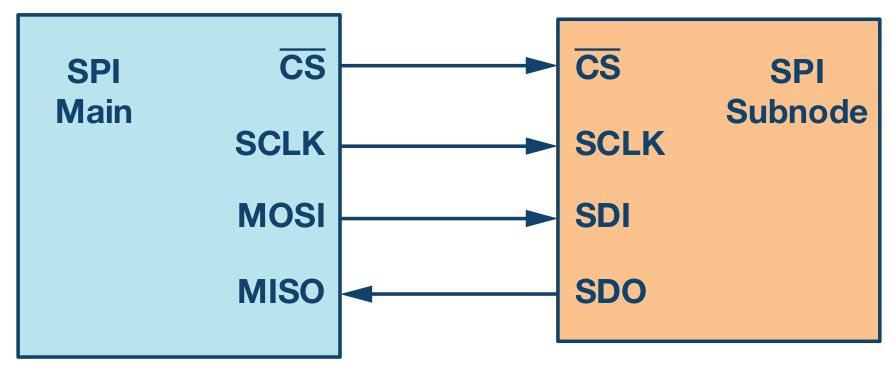
\includegraphics[width=0.6\textwidth]{./Figures/SPI.png}
	\caption{Conexión entre dispositivos SPI.\protect\footnotemark.}
	\label{fig:SPI}
\end{figure} 

Los dispositivos SPI pueden ser direccionables mediante las señales de CS \textit{chip select} y alcanzar velocidades de reloj de hasta 50MHz. 

Esto permite la comunicación entre dispositivos que transfieren un gran cantidad de datos como displays, modulos ethernet y memorias entre otros. 


\subsection{I2C \textit{Inter Integrated Circuit}}

I2C es un protocolo de comunicación serie  bidireccional con un número reducido de hilos para su conexión. Como puede observarse en la figura \ref{fig:I2C}, solo se necesitan dos cables para conectar una serie de dispositivos.

\begin{figure}[htbp]
	\centering
	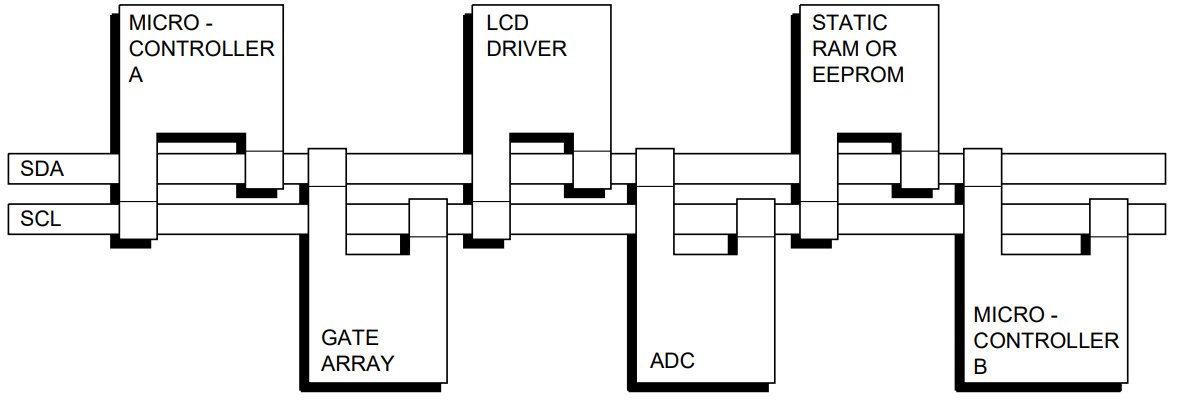
\includegraphics[width=0.8\textwidth]{./Figures/I2C.png}
	\caption{Conexión entre dispositivos I2C.\protect\footnotemark.}
	\label{fig:I2C}
\end{figure} 

Soporta un rango de velocidades desde los 100 kHz a los 5MHz, es direccionable y cuenta con dispositivos para aplicaciones, militares, medicinales e industriales.

Entre los más utilizados se pueden encontrar, memorias, ADC, DAC, sensores de temperatura y humedad, giróscopos electrónicos, etc.

\subsection{UART \textit{Universal Asincronous Receiver Transmitter}}

El protocolo de comunicación serie UART es uno de los más antiguos y utilizados en la comunicación entre dispositivos. Este protocolo es asincrónico, por lo que no cuenta una señal de clock, esta característica reduce la cantidad de hilos de conexión como se detalla en la Figura \ref{fig:UART}


\begin{figure}[htbp]
	\centering
	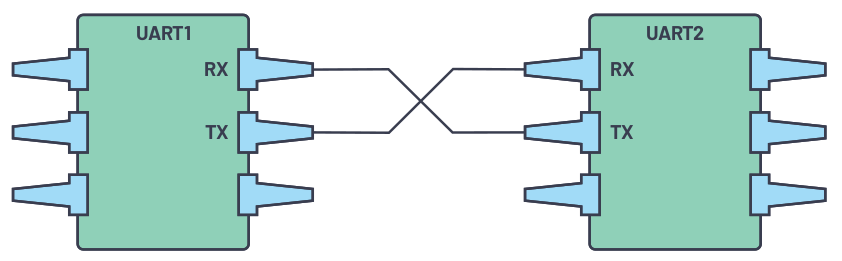
\includegraphics[width=0.6\textwidth]{./Figures/UART.png}
	\caption{Conexión entre dispositivos UART.\protect\footnotemark.}
	\label{fig:UART}
\end{figure} 

A diferencias de los protocolos I2C y  SPI, este no soporta direccionamiento, y su velocidad de comunicación es muy inferior en comparación a los anteriores. Dedido a su sencillez y bajo costo el mismo se continúa utilizando en algunos dispositivos como, módulos WiFi, módulos LoRa, interfaz de comunicación a PC e impresoras.

\subsection{LoRa \textit{Long Range}}

LoRa es una tecnología de comunicación inalámbrica que utiliza la modulación CSS(\textit{Chip Spread Spectrum}) desarrollada por la empresa Semtech. 
La utilización de este tipo de modulación posee grandes ventajas de alcance, inmunidad al ruido y consumo.
En la figura \ref{fig:LoRa} se observa la forma de onda modulada de un dispositivo LoRa. 

\begin{figure}[htbp]
	\centering
	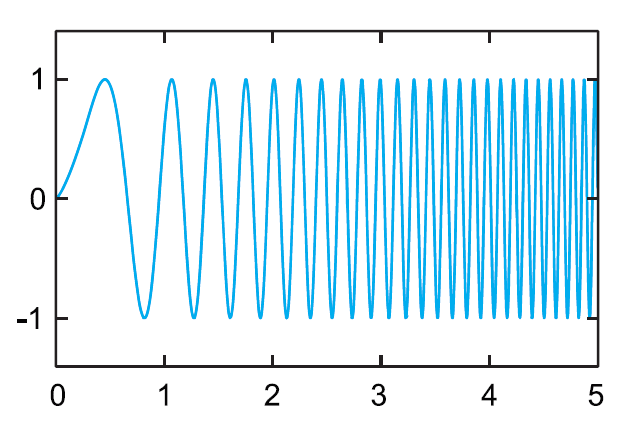
\includegraphics[width=0.3\textwidth]{./Figures/LoRa.png}
	\caption{Modulación CSS.\protect\footnotemark.}
	\label{fig:LoRa}
\end{figure} 

Los dispositivos LoRa utilizan el espectro de frecuencias no licenciado ISM ( \textit{Industrial, Scientific and Medical}) de 915 MHz para el caso de nuestro país, esto reduce el costo operativo de la instalación de dispositivos con esta tecnología.

Con la incorporación del \textit{stack} LoRaWAN, esta tecnología se ha convertido en una de las mas populares en el ecosistema IoT.


\subsection{ModBUS TCP}

Modbus es un protocolo de aplicación abierto Maestro/Esclavo que se puede utilizar en distintas capas físicas. 
Modbus TCP significa que el protocolo Modbus se utiliza en la parte superior de Ethernet TCP/IP, un protocolo orientado a la conexión con el que se busca asegurar la entrega de datos.

\begin{figure}[htbp]
	\centering
	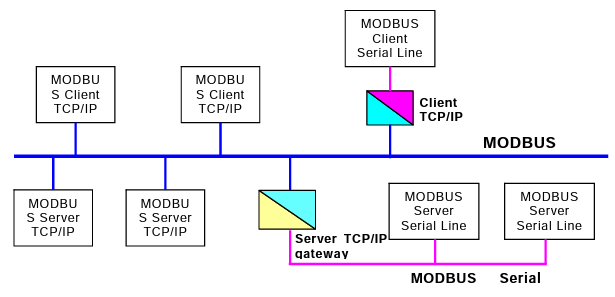
\includegraphics[width=0.7\textwidth]{./Figures/ModBUS.png}
	\caption{Arquitectura de comunicación ModBUS TCP.\protect\footnotemark.}
	\label{fig:ModBUS}
\end{figure} 

Este protocolo ha sido adoptado en la industria por una gran cantidad de fabricantes y en dispositivos controladores lógicos programables, interfase hombre máquina, sensores, actuadores, variadores de velocidad, etc.

ModBUS es un protocolo sencillo, económico y de rápida implementación. Dada su integración existente en los distintos componentes industriales, es muy utilizado cuando se requiere obtener datos de dispositivos industriales. 

\subsection{HTTP \textit{Hypertext Transfer Protocol}}

HTTP es un protocolo de la capa de aplicación para la transmisión de documentos hipermedia, como HTML \textit{HyperText Markup Language} del tipo cliente - servidor. 
Es un protocolo del tipo cliente - servidor, en el que un cliente establece una conexión con el servidor, realiza una petición y espera hasta que recibe una respuesta.

\subsection{Wi-Fi}

\subsection{MQTT}


%\subsection{Uso de mayúscula inicial para los título de secciones}

Si en el texto se hace alusión a diferentes partes del trabajo referirse a ellas como capítulo, sección o subsección según corresponda. Por ejemplo: ``En el capítulo \ref{Chapter1} se explica tal cosa'', o ``En la sección \ref{sec:ejemplo} se presenta lo que sea'', o ``En la subsección \ref{subsec:ejemplo} se discute otra cosa''.

Cuando se quiere poner una lista tabulada, se hace así:

\begin{itemize}
	\item Este es el primer elemento de la lista.
	\item Este es el segundo elemento de la lista.
\end{itemize}

Notar el uso de las mayúsculas y el punto al final de cada elemento.

Si se desea poner una lista numerada el formato es este:

\begin{enumerate}
	\item Este es el primer elemento de la lista.
	\item Este es el segundo elemento de la lista.
\end{enumerate}

Notar el uso de las mayúsculas y el punto al final de cada elemento.

\section{Tecnologías de backend}
\label{subsec:ejemplo}

Se recomienda no utilizar \textbf{texto en negritas} en ningún párrafo, ni tampoco texto \underline{subrayado}. En cambio sí se debe utilizar \textit{texto en itálicas} para palabras en un idioma extranjero, al menos la primera vez que aparecen en el texto. En el caso de palabras que estamos inventando se deben utilizar ``comillas'', así como también para citas textuales. Por ejemplo, un \textit{digital filter} es una especie de ``selector'' que permite separar ciertos componentes armónicos en particular.

La escritura debe ser impersonal. Por ejemplo, no utilizar ``el diseño del firmware lo hice de acuerdo con tal principio'', sino ``el firmware fue diseñado utilizando tal principio''. 

El trabajo es algo que al momento de escribir la memoria se supone que ya está concluido, entonces todo lo que se refiera a hacer el trabajo se narra en tiempo pasado, porque es algo que ya ocurrió. Por ejemplo, "se diseñó el firmware empleando la técnica de test driven development".

En cambio, la memoria es algo que está vivo cada vez que el lector la lee. Por eso transcurre siempre en tiempo presente, como por ejemplo:

``En el presente capítulo se da una visión global sobre las distintas pruebas realizadas y los resultados obtenidos. Se explica el modo en que fueron llevados a cabo los test unitarios y las pruebas del sistema''.

Se recomienda no utilizar una sección de glosario sino colocar la descripción de las abreviaturas como parte del mismo cuerpo del texto. Por ejemplo, RTOS (\textit{Real Time Operating System}, Sistema Operativo de Tiempo Real) o en caso de considerarlo apropiado mediante notas a pie de página.

Si se desea indicar alguna página web utilizar el siguiente formato de referencias bibliográficas, dónde las referencias se detallan en la sección de bibliografía de la memoria, utilizado el formato establecido por IEEE en \citep{IEEE:citation}. Por ejemplo, ``el presente trabajo se basa en la plataforma EDU-CIAA-NXP \citep{CIAA}, la cual...''.

\section{Tecnologías de frontend} 

Al insertar figuras en la memoria se deben considerar determinadas pautas. Para empezar, usar siempre tipografía claramente legible. Luego, tener claro que \textbf{es incorrecto} escribir por ejemplo esto: ``El diseño elegido es un cuadrado, como se ve en la siguiente figura:''

\begin{figure}[h]
\centering
\includegraphics[scale=.45]{./Figures/cuadradoAzul.png}
\end{figure}

La forma correcta de utilizar una figura es con referencias cruzadas, por ejemplo: ``Se eligió utilizar un cuadrado azul para el logo, como puede observarse en la figura \ref{fig:cuadradoAzul}''.

\begin{figure}[ht]
	\centering
	\includegraphics[scale=.45]{./Figures/cuadradoAzul.png}
	\caption{Ilustración del cuadrado azul que se eligió para el diseño del logo.}
	\label{fig:cuadradoAzul}
\end{figure}

El texto de las figuras debe estar siempre en español, excepto que se decida reproducir una figura original tomada de alguna referencia. En ese caso la referencia de la cual se tomó la figura debe ser indicada en el epígrafe de la figura e incluida como una nota al pie, como se ilustra en la figura \ref{fig:palabraIngles}.

\begin{figure}[htpb]
	\centering
	\includegraphics[scale=.3]{./Figures/word.jpeg}
	\caption{Imagen tomada de la página oficial del procesador\protect\footnotemark.}
	\label{fig:palabraIngles}
\end{figure}

\footnotetext{Imagen tomada de \url{https://goo.gl/images/i7C70w}}

La figura y el epígrafe deben conformar una unidad cuyo significado principal pueda ser comprendido por el lector sin necesidad de leer el cuerpo central de la memoria. Para eso es necesario que el epígrafe sea todo lo detallado que corresponda y si en la figura se utilizan abreviaturas entonces aclarar su significado en el epígrafe o en la misma figura.



\begin{figure}[ht]
	\centering
	\includegraphics[scale=.37]{./Figures/questionMark.png}
	\caption{¿Por qué de pronto aparece esta figura?}
	\label{fig:questionMark}
\end{figure}

Nunca colocar una figura en el documento antes de hacer la primera referencia a ella, como se ilustra con la figura \ref{fig:questionMark}, porque sino el lector no comprenderá por qué de pronto aparece la figura en el documento, lo que distraerá su atención.

Otra posibilidad es utilizar el entorno \textit{subfigure} para incluir más de una figura, como se puede ver en la figura \ref{fig:three graphs}. Notar que se pueden referenciar también las figuras internas individualmente de esta manera: \ref{fig:1de3}, \ref{fig:2de3} y \ref{fig:3de3}.
 
\begin{figure}[!htpb]
     \centering
     \begin{subfigure}[b]{0.3\textwidth}
         \centering
         \includegraphics[width=.65\textwidth]{./Figures/questionMark}
         \caption{Un caption.}
         \label{fig:1de3}
     \end{subfigure}
     \hfill
     \begin{subfigure}[b]{0.3\textwidth}
         \centering
         \includegraphics[width=.65\textwidth]{./Figures/questionMark}
         \caption{Otro.}
         \label{fig:2de3}
     \end{subfigure}
     \hfill
     \begin{subfigure}[b]{0.3\textwidth}
         \centering
         \includegraphics[width=.65\textwidth]{./Figures/questionMark}
         \caption{Y otro más.}
         \label{fig:3de3}
     \end{subfigure}
        \caption{Tres gráficos simples}
        \label{fig:three graphs}
\end{figure}

El código para generar las imágenes se encuentra disponible para su reutilización en el archivo \file{Chapter2.tex}.

\section{Dispositivos Bare Metal}

Para las tablas utilizar el mismo formato que para las figuras, sólo que el epígrafe se debe colocar arriba de la tabla, como se ilustra en la tabla \ref{tab:peces}. Observar que sólo algunas filas van con líneas visibles y notar el uso de las negritas para los encabezados.  La referencia se logra utilizando el comando \verb|\ref{<label>}| donde label debe estar definida dentro del entorno de la tabla.

\begin{verbatim}
\begin{table}[h]
	\centering
	\caption[caption corto]{caption largo más descriptivo}
	\begin{tabular}{l c c}    
		\toprule
		\textbf{Especie}     & \textbf{Tamaño} & \textbf{Valor}\\
		\midrule
		Amphiprion Ocellaris & 10 cm           & \$ 6.000 \\		
		Hepatus Blue Tang    & 15 cm           & \$ 7.000 \\
		Zebrasoma Xanthurus  & 12 cm           & \$ 6.800 \\
		\bottomrule
		\hline
	\end{tabular}
	\label{tab:peces}
\end{table}
\end{verbatim}


\begin{table}[h]
	\centering
	\caption[caption corto]{caption largo más descriptivo}
	\begin{tabular}{l c c}    
		\toprule
		\textbf{Especie} 	 & \textbf{Tamaño} 		& \textbf{Valor}  \\
		\midrule
		Amphiprion Ocellaris & 10 cm 				& \$ 6.000 \\		
		Hepatus Blue Tang	 & 15 cm				& \$ 7.000 \\
		Zebrasoma Xanthurus	 & 12 cm				& \$ 6.800 \\
		\bottomrule
		\hline
	\end{tabular}
	\label{tab:peces}
\end{table}

En cada capítulo se debe reiniciar el número de conteo de las figuras y las tablas, por ejemplo, figura 2.1 o tabla 2.1, pero no se debe reiniciar el conteo en cada sección. Por suerte la plantilla se encarga de esto por nosotros.

\section{Herramientas utilizadas}
\label{sec:Ecuaciones}

Al insertar ecuaciones en la memoria dentro de un entorno \textit{equation}, éstas se numeran en forma automática  y se pueden referir al igual que como se hace con las figuras y tablas, por ejemplo ver la ecuación \ref{eq:metric}.

\begin{equation}
	\label{eq:metric}
	ds^2 = c^2 dt^2 \left( \frac{d\sigma^2}{1-k\sigma^2} + \sigma^2\left[ d\theta^2 + \sin^2\theta d\phi^2 \right] \right)
\end{equation}
                                                        
Es importante tener presente que si bien las ecuaciones pueden ser referidas por su número, también es correcto utilizar los dos puntos, como por ejemplo ``la expresión matemática que describe este comportamiento es la siguiente:''

\begin{equation}
	\label{eq:schrodinger}
	\frac{\hbar^2}{2m}\nabla^2\Psi + V(\mathbf{r})\Psi = -i\hbar \frac{\partial\Psi}{\partial t}
\end{equation}

Para generar la ecuación \ref{eq:metric} se utilizó el siguiente código:

\begin{verbatim}
\begin{equation}
	\label{eq:metric}
	ds^2 = c^2 dt^2 \left( \frac{d\sigma^2}{1-k\sigma^2} + 
	\sigma^2\left[ d\theta^2 + 
	\sin^2\theta d\phi^2 \right] \right)
\end{equation}
\end{verbatim}

Y para la ecuación \ref{eq:schrodinger}:

\begin{verbatim}
\begin{equation}
	\label{eq:schrodinger}
	\frac{\hbar^2}{2m}\nabla^2\Psi + V(\mathbf{r})\Psi = 
	-i\hbar \frac{\partial\Psi}{\partial t}
\end{equation}

\end{verbatim} 
%	\include{Chapters/Chapter3}
%	\include{Chapters/Chapter4} 
%	\include{Chapters/Chapter5} 
%\end{verbatim}
%
%Los apéndices también deben escribirse en archivos .tex separados, que se deben ubicar dentro de la carpeta \emph{Appendices}. Los apéndices vienen comentados por defecto con el caracter \code{\%} y para incluirlos simplemente se debe eliminar dicho caracter.
%
%Finalmente, se encuentra el código para incluir la bibliografía en el documento final.  Este código tampoco debe modificarse. La metodología para trabajar las referencias bibliográficas se desarrolla en la sección \ref{sec:biblio}.
%----------------------------------------------------------------------------------------

%\section{Bibliografía}
%\label{sec:biblio}
%
%Las opciones de formato de la bibliografía se controlan a través del paquete de latex \option{biblatex} que se incluye en la memoria en el archivo memoria.tex.  Estas opciones determinan cómo se generan las citas bibliográficas en el cuerpo del documento y cómo se genera la bibliografía al final de la memoria.
%
%En el preámbulo se puede encontrar el código que incluye el paquete biblatex, que no requiere ninguna modificación del usuario de la plantilla, y que contiene las siguientes opciones:
%
%\begin{lstlisting}
%\usepackage[backend=bibtex,
%	natbib=true, 
%	style=numeric, 
%	sorting=none]
%{biblatex}
%\end{lstlisting}
%
%En el archivo \file{reference.bib} se encuentran las referencias bibliográficas que se pueden citar en el documento.  Para incorporar una nueva cita al documento lo primero es agregarla en este archivo con todos los campos necesario.  Todas las entradas bibliográficas comienzan con $@$ y una palabra que define el formato de la entrada.  Para cada formato existen campos obligatorios que deben completarse. No importa el orden en que las entradas estén definidas en el archivo .bib.  Tampoco es importante el orden en que estén definidos los campos de una entrada bibliográfica. A continuación se muestran algunos ejemplos:
%
%\begin{lstlisting}
%@ARTICLE{ARTICLE:1,
%    AUTHOR="John Doe",
%    TITLE="Title",
%    JOURNAL="Journal",
%    YEAR="2017",
%}
%\end{lstlisting}
%
%
%\begin{lstlisting}
%@BOOK{BOOK:1,
%    AUTHOR="John Doe",
%    TITLE="The Book without Title",
%    PUBLISHER="Dummy Publisher",
%    YEAR="2100",
%}
%\end{lstlisting}
%
%
%\begin{lstlisting}
%@INBOOK{BOOK:2,
%    AUTHOR="John Doe",
%    TITLE="The Book without Title",
%    PUBLISHER="Dummy Publisher",
%    YEAR="2100",
%    PAGES="100-200",
%}
%\end{lstlisting}
%
%
%\begin{lstlisting}
%@MISC{WEBSITE:1,
%    HOWPUBLISHED = "\url{http://example.com}",
%    AUTHOR = "Intel",
%    TITLE = "Example Website",
%    MONTH = "12",
%    YEAR = "1988",
%    URLDATE = {2012-11-26}
%}
%\end{lstlisting}
%
%Se debe notar que los nombres \emph{ARTICLE:1}, \emph{BOOK:1}, \emph{BOOK:2} y \emph{WEBSITE:1} son nombres de fantasía que le sirve al autor del documento para identificar la entrada. En este sentido, se podrían reemplazar por cualquier otro nombre.  Tampoco es necesario poner : seguido de un número, en los ejemplos sólo se incluye como un posible estilo para identificar las entradas.
%
%La entradas se citan en el documento con el comando: 
%
%\begin{verbatim}
%\citep{nombre_de_la_entrada}
%\end{verbatim}
%
%Y cuando se usan, se muestran así: \citep{ARTICLE:1}, \citep{BOOK:1}, \citep{BOOK:2}, \citep{WEBSITE:1}.  Notar cómo se conforma la sección Bibliografía al final del documento.
%
%Finalmente y como se mencionó en la subsección \ref{subsec:configurando}, para actualizar las referencias bibliográficas tanto en la sección bibliografía como las citas en el cuerpo del documento, se deben ejecutar las herramientas de compilación PDFLaTeX, BibTeX, PDFLaTeX, PDFLaTeX, en ese orden.  Este procedimiento debería resolver cualquier mensaje "Citation xxxxx on page x undefined".

%\chapter{Introducción específica} % Main chapter title

\label{Chapter2}

%----------------------------------------------------------------------------------------
%	SECTION 1
%----------------------------------------------------------------------------------------
En el siguiente capitulo se realiza una introducción a las tecnológicas utilizadas en el desarrollo de este trabajo. Estas tecnologías se aplican a lo largo de las distintas capas del modelo de arquitectura IoT (\textit{Internet of Things})
\section{Protocolos de comunicación}
\label{sec:ejemplo}

Los protocolos de comunicación son estándares que se utilizar para definir de que manera se vinculan uno o mas dispositivos. Existen una gran cantidad de protocolos, estos resuelven distintas problemáticas, a continuación se detallan los utilizados en el desarrollo de este trabajo.

\subsection{SPI \textit{Serial Peripherical Interface}}

EL protocolo de comunicación SPI es un protocolo de comunicación serie que se caracteriza por ser sincrónico y \textit{full duplex}.
Su comunicación se realiza mediante 4 hilos como se observa en la figura \ref{fig:SPI} .

\begin{figure}[htbp]
	\centering
	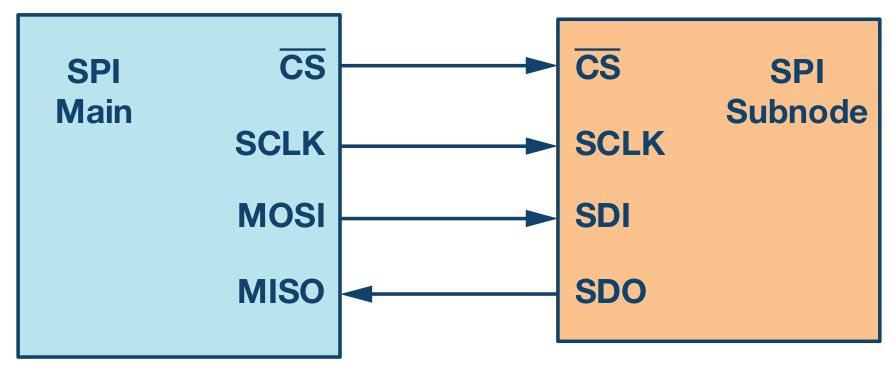
\includegraphics[width=0.6\textwidth]{./Figures/SPI.png}
	\caption{Conexión entre dispositivos SPI.\protect\footnotemark.}
	\label{fig:SPI}
\end{figure} 

Los dispositivos SPI pueden ser direccionables mediante las señales de CS \textit{chip select} y alcanzar velocidades de reloj de hasta 50MHz. 

Esto permite la comunicación entre dispositivos que transfieren un gran cantidad de datos como displays, modulos ethernet y memorias entre otros. 


\subsection{I2C \textit{Inter Integrated Circuit}}

I2C es un protocolo de comunicación serie  bidireccional con un número reducido de hilos para su conexión. Como puede observarse en la figura \ref{fig:I2C}, solo se necesitan dos cables para conectar una serie de dispositivos.

\begin{figure}[htbp]
	\centering
	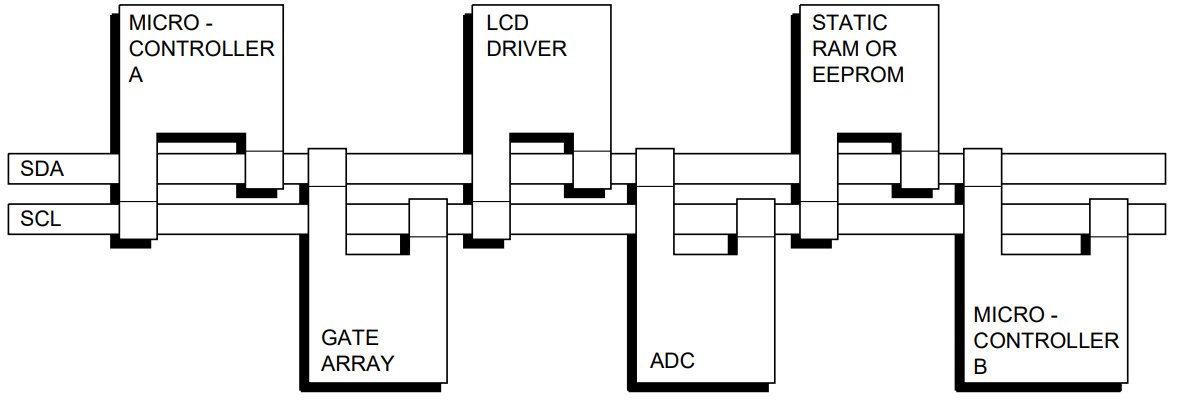
\includegraphics[width=0.8\textwidth]{./Figures/I2C.png}
	\caption{Conexión entre dispositivos I2C.\protect\footnotemark.}
	\label{fig:I2C}
\end{figure} 

Soporta un rango de velocidades desde los 100 kHz a los 5MHz, es direccionable y cuenta con dispositivos para aplicaciones, militares, medicinales e industriales.

Entre los más utilizados se pueden encontrar, memorias, ADC, DAC, sensores de temperatura y humedad, giróscopos electrónicos, etc.

\subsection{UART \textit{Universal Asincronous Receiver Transmitter}}

El protocolo de comunicación serie UART es uno de los más antiguos y utilizados en la comunicación entre dispositivos. Este protocolo es asincrónico, por lo que no cuenta una señal de clock, esta característica reduce la cantidad de hilos de conexión como se detalla en la Figura \ref{fig:UART}


\begin{figure}[htbp]
	\centering
	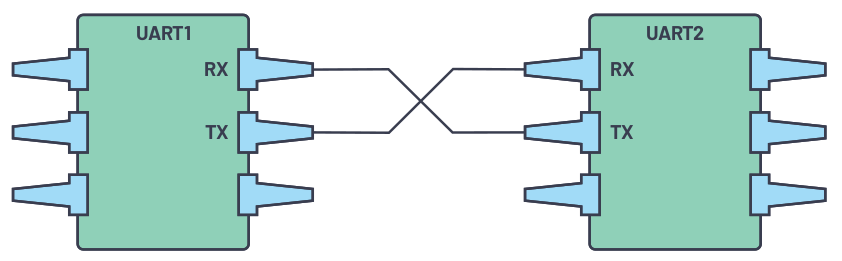
\includegraphics[width=0.6\textwidth]{./Figures/UART.png}
	\caption{Conexión entre dispositivos UART.\protect\footnotemark.}
	\label{fig:UART}
\end{figure} 

A diferencias de los protocolos I2C y  SPI, este no soporta direccionamiento, y su velocidad de comunicación es muy inferior en comparación a los anteriores. Dedido a su sencillez y bajo costo el mismo se continúa utilizando en algunos dispositivos como, módulos WiFi, módulos LoRa, interfaz de comunicación a PC e impresoras.

\subsection{LoRa \textit{Long Range}}

LoRa es una tecnología de comunicación inalámbrica que utiliza la modulación CSS(\textit{Chip Spread Spectrum}) desarrollada por la empresa Semtech. 
La utilización de este tipo de modulación posee grandes ventajas de alcance, inmunidad al ruido y consumo.
En la figura \ref{fig:LoRa} se observa la forma de onda modulada de un dispositivo LoRa. 

\begin{figure}[htbp]
	\centering
	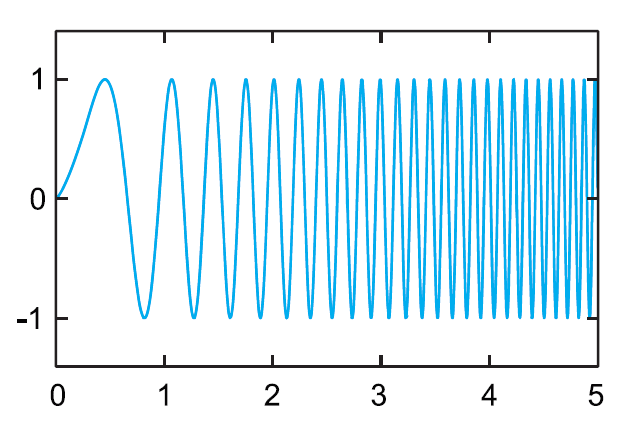
\includegraphics[width=0.3\textwidth]{./Figures/LoRa.png}
	\caption{Modulación CSS.\protect\footnotemark.}
	\label{fig:LoRa}
\end{figure} 

Los dispositivos LoRa utilizan el espectro de frecuencias no licenciado ISM ( \textit{Industrial, Scientific and Medical}) de 915 MHz para el caso de nuestro país, esto reduce el costo operativo de la instalación de dispositivos con esta tecnología.

Con la incorporación del \textit{stack} LoRaWAN, esta tecnología se ha convertido en una de las mas populares en el ecosistema IoT.


\subsection{ModBUS TCP}

Modbus es un protocolo de aplicación abierto Maestro/Esclavo que se puede utilizar en distintas capas físicas. 
Modbus TCP significa que el protocolo Modbus se utiliza en la parte superior de Ethernet TCP/IP, un protocolo orientado a la conexión con el que se busca asegurar la entrega de datos.

\begin{figure}[htbp]
	\centering
	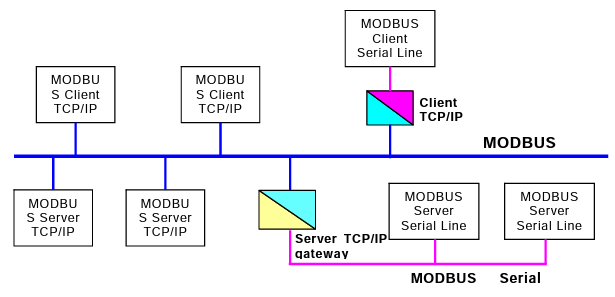
\includegraphics[width=0.7\textwidth]{./Figures/ModBUS.png}
	\caption{Arquitectura de comunicación ModBUS TCP.\protect\footnotemark.}
	\label{fig:ModBUS}
\end{figure} 

Este protocolo ha sido adoptado en la industria por una gran cantidad de fabricantes y en dispositivos controladores lógicos programables, interfase hombre máquina, sensores, actuadores, variadores de velocidad, etc.

ModBUS es un protocolo sencillo, económico y de rápida implementación. Dada su integración existente en los distintos componentes industriales, es muy utilizado cuando se requiere obtener datos de dispositivos industriales. 

\subsection{HTTP \textit{Hypertext Transfer Protocol}}

HTTP es un protocolo de la capa de aplicación para la transmisión de documentos hipermedia, como HTML \textit{HyperText Markup Language} del tipo cliente - servidor. 
Es un protocolo del tipo cliente - servidor, en el que un cliente establece una conexión con el servidor, realiza una petición y espera hasta que recibe una respuesta.

\subsection{Wi-Fi}

\subsection{MQTT}


%\subsection{Uso de mayúscula inicial para los título de secciones}

Si en el texto se hace alusión a diferentes partes del trabajo referirse a ellas como capítulo, sección o subsección según corresponda. Por ejemplo: ``En el capítulo \ref{Chapter1} se explica tal cosa'', o ``En la sección \ref{sec:ejemplo} se presenta lo que sea'', o ``En la subsección \ref{subsec:ejemplo} se discute otra cosa''.

Cuando se quiere poner una lista tabulada, se hace así:

\begin{itemize}
	\item Este es el primer elemento de la lista.
	\item Este es el segundo elemento de la lista.
\end{itemize}

Notar el uso de las mayúsculas y el punto al final de cada elemento.

Si se desea poner una lista numerada el formato es este:

\begin{enumerate}
	\item Este es el primer elemento de la lista.
	\item Este es el segundo elemento de la lista.
\end{enumerate}

Notar el uso de las mayúsculas y el punto al final de cada elemento.

\section{Tecnologías de backend}
\label{subsec:ejemplo}

Se recomienda no utilizar \textbf{texto en negritas} en ningún párrafo, ni tampoco texto \underline{subrayado}. En cambio sí se debe utilizar \textit{texto en itálicas} para palabras en un idioma extranjero, al menos la primera vez que aparecen en el texto. En el caso de palabras que estamos inventando se deben utilizar ``comillas'', así como también para citas textuales. Por ejemplo, un \textit{digital filter} es una especie de ``selector'' que permite separar ciertos componentes armónicos en particular.

La escritura debe ser impersonal. Por ejemplo, no utilizar ``el diseño del firmware lo hice de acuerdo con tal principio'', sino ``el firmware fue diseñado utilizando tal principio''. 

El trabajo es algo que al momento de escribir la memoria se supone que ya está concluido, entonces todo lo que se refiera a hacer el trabajo se narra en tiempo pasado, porque es algo que ya ocurrió. Por ejemplo, "se diseñó el firmware empleando la técnica de test driven development".

En cambio, la memoria es algo que está vivo cada vez que el lector la lee. Por eso transcurre siempre en tiempo presente, como por ejemplo:

``En el presente capítulo se da una visión global sobre las distintas pruebas realizadas y los resultados obtenidos. Se explica el modo en que fueron llevados a cabo los test unitarios y las pruebas del sistema''.

Se recomienda no utilizar una sección de glosario sino colocar la descripción de las abreviaturas como parte del mismo cuerpo del texto. Por ejemplo, RTOS (\textit{Real Time Operating System}, Sistema Operativo de Tiempo Real) o en caso de considerarlo apropiado mediante notas a pie de página.

Si se desea indicar alguna página web utilizar el siguiente formato de referencias bibliográficas, dónde las referencias se detallan en la sección de bibliografía de la memoria, utilizado el formato establecido por IEEE en \citep{IEEE:citation}. Por ejemplo, ``el presente trabajo se basa en la plataforma EDU-CIAA-NXP \citep{CIAA}, la cual...''.

\section{Tecnologías de frontend} 

Al insertar figuras en la memoria se deben considerar determinadas pautas. Para empezar, usar siempre tipografía claramente legible. Luego, tener claro que \textbf{es incorrecto} escribir por ejemplo esto: ``El diseño elegido es un cuadrado, como se ve en la siguiente figura:''

\begin{figure}[h]
\centering
\includegraphics[scale=.45]{./Figures/cuadradoAzul.png}
\end{figure}

La forma correcta de utilizar una figura es con referencias cruzadas, por ejemplo: ``Se eligió utilizar un cuadrado azul para el logo, como puede observarse en la figura \ref{fig:cuadradoAzul}''.

\begin{figure}[ht]
	\centering
	\includegraphics[scale=.45]{./Figures/cuadradoAzul.png}
	\caption{Ilustración del cuadrado azul que se eligió para el diseño del logo.}
	\label{fig:cuadradoAzul}
\end{figure}

El texto de las figuras debe estar siempre en español, excepto que se decida reproducir una figura original tomada de alguna referencia. En ese caso la referencia de la cual se tomó la figura debe ser indicada en el epígrafe de la figura e incluida como una nota al pie, como se ilustra en la figura \ref{fig:palabraIngles}.

\begin{figure}[htpb]
	\centering
	\includegraphics[scale=.3]{./Figures/word.jpeg}
	\caption{Imagen tomada de la página oficial del procesador\protect\footnotemark.}
	\label{fig:palabraIngles}
\end{figure}

\footnotetext{Imagen tomada de \url{https://goo.gl/images/i7C70w}}

La figura y el epígrafe deben conformar una unidad cuyo significado principal pueda ser comprendido por el lector sin necesidad de leer el cuerpo central de la memoria. Para eso es necesario que el epígrafe sea todo lo detallado que corresponda y si en la figura se utilizan abreviaturas entonces aclarar su significado en el epígrafe o en la misma figura.



\begin{figure}[ht]
	\centering
	\includegraphics[scale=.37]{./Figures/questionMark.png}
	\caption{¿Por qué de pronto aparece esta figura?}
	\label{fig:questionMark}
\end{figure}

Nunca colocar una figura en el documento antes de hacer la primera referencia a ella, como se ilustra con la figura \ref{fig:questionMark}, porque sino el lector no comprenderá por qué de pronto aparece la figura en el documento, lo que distraerá su atención.

Otra posibilidad es utilizar el entorno \textit{subfigure} para incluir más de una figura, como se puede ver en la figura \ref{fig:three graphs}. Notar que se pueden referenciar también las figuras internas individualmente de esta manera: \ref{fig:1de3}, \ref{fig:2de3} y \ref{fig:3de3}.
 
\begin{figure}[!htpb]
     \centering
     \begin{subfigure}[b]{0.3\textwidth}
         \centering
         \includegraphics[width=.65\textwidth]{./Figures/questionMark}
         \caption{Un caption.}
         \label{fig:1de3}
     \end{subfigure}
     \hfill
     \begin{subfigure}[b]{0.3\textwidth}
         \centering
         \includegraphics[width=.65\textwidth]{./Figures/questionMark}
         \caption{Otro.}
         \label{fig:2de3}
     \end{subfigure}
     \hfill
     \begin{subfigure}[b]{0.3\textwidth}
         \centering
         \includegraphics[width=.65\textwidth]{./Figures/questionMark}
         \caption{Y otro más.}
         \label{fig:3de3}
     \end{subfigure}
        \caption{Tres gráficos simples}
        \label{fig:three graphs}
\end{figure}

El código para generar las imágenes se encuentra disponible para su reutilización en el archivo \file{Chapter2.tex}.

\section{Dispositivos Bare Metal}

Para las tablas utilizar el mismo formato que para las figuras, sólo que el epígrafe se debe colocar arriba de la tabla, como se ilustra en la tabla \ref{tab:peces}. Observar que sólo algunas filas van con líneas visibles y notar el uso de las negritas para los encabezados.  La referencia se logra utilizando el comando \verb|\ref{<label>}| donde label debe estar definida dentro del entorno de la tabla.

\begin{verbatim}
\begin{table}[h]
	\centering
	\caption[caption corto]{caption largo más descriptivo}
	\begin{tabular}{l c c}    
		\toprule
		\textbf{Especie}     & \textbf{Tamaño} & \textbf{Valor}\\
		\midrule
		Amphiprion Ocellaris & 10 cm           & \$ 6.000 \\		
		Hepatus Blue Tang    & 15 cm           & \$ 7.000 \\
		Zebrasoma Xanthurus  & 12 cm           & \$ 6.800 \\
		\bottomrule
		\hline
	\end{tabular}
	\label{tab:peces}
\end{table}
\end{verbatim}


\begin{table}[h]
	\centering
	\caption[caption corto]{caption largo más descriptivo}
	\begin{tabular}{l c c}    
		\toprule
		\textbf{Especie} 	 & \textbf{Tamaño} 		& \textbf{Valor}  \\
		\midrule
		Amphiprion Ocellaris & 10 cm 				& \$ 6.000 \\		
		Hepatus Blue Tang	 & 15 cm				& \$ 7.000 \\
		Zebrasoma Xanthurus	 & 12 cm				& \$ 6.800 \\
		\bottomrule
		\hline
	\end{tabular}
	\label{tab:peces}
\end{table}

En cada capítulo se debe reiniciar el número de conteo de las figuras y las tablas, por ejemplo, figura 2.1 o tabla 2.1, pero no se debe reiniciar el conteo en cada sección. Por suerte la plantilla se encarga de esto por nosotros.

\section{Herramientas utilizadas}
\label{sec:Ecuaciones}

Al insertar ecuaciones en la memoria dentro de un entorno \textit{equation}, éstas se numeran en forma automática  y se pueden referir al igual que como se hace con las figuras y tablas, por ejemplo ver la ecuación \ref{eq:metric}.

\begin{equation}
	\label{eq:metric}
	ds^2 = c^2 dt^2 \left( \frac{d\sigma^2}{1-k\sigma^2} + \sigma^2\left[ d\theta^2 + \sin^2\theta d\phi^2 \right] \right)
\end{equation}
                                                        
Es importante tener presente que si bien las ecuaciones pueden ser referidas por su número, también es correcto utilizar los dos puntos, como por ejemplo ``la expresión matemática que describe este comportamiento es la siguiente:''

\begin{equation}
	\label{eq:schrodinger}
	\frac{\hbar^2}{2m}\nabla^2\Psi + V(\mathbf{r})\Psi = -i\hbar \frac{\partial\Psi}{\partial t}
\end{equation}

Para generar la ecuación \ref{eq:metric} se utilizó el siguiente código:

\begin{verbatim}
\begin{equation}
	\label{eq:metric}
	ds^2 = c^2 dt^2 \left( \frac{d\sigma^2}{1-k\sigma^2} + 
	\sigma^2\left[ d\theta^2 + 
	\sin^2\theta d\phi^2 \right] \right)
\end{equation}
\end{verbatim}

Y para la ecuación \ref{eq:schrodinger}:

\begin{verbatim}
\begin{equation}
	\label{eq:schrodinger}
	\frac{\hbar^2}{2m}\nabla^2\Psi + V(\mathbf{r})\Psi = 
	-i\hbar \frac{\partial\Psi}{\partial t}
\end{equation}

\end{verbatim} 
%\include{Chapters/Chapter3}
%\include{Chapters/Chapter4} 
%\include{Chapters/Chapter5} 

%----------------------------------------------------------------------------------------
%	CONTENIDO DE LA MEMORIA  - APÉNDICES
%----------------------------------------------------------------------------------------

\appendix % indicativo para indicarle a LaTeX los siguientes "capítulos" son apéndices

% Incluir los apéndices de la memoria como archivos separadas desde la carpeta Appendices
% Descomentar las líneas a medida que se escriben los apéndices

%\include{Appendices/AppendixA}
%\include{Appendices/AppendixB}
%\include{Appendices/AppendixC}

%----------------------------------------------------------------------------------------
%	BIBLIOGRAPHY
%----------------------------------------------------------------------------------------

\Urlmuskip=0mu plus 1mu\relax
\raggedright
\printbibliography[heading=bibintoc]

%----------------------------------------------------------------------------------------

\end{document}  
